% Lines starting with a percent sign (%) are comments. LaTeX will 
% not process those lines. Similarly, everything after a percent 
% sign in a line is considered a comment. To produce a percent sign
% in the output, write \% (backslash followed by the percent sign). 
% ==================================================================
% Usage instructions:
% ------------------------------------------------------------------
% The file is heavily commented so that you know what the various
% commands do. Feel free to remove any comments you don't need from
% your own copy. When redistributing the example thesis file, please
% retain all the comments for the benefit of other thesis writers! 
% ==================================================================
% Compilation instructions: 
% ------------------------------------------------------------------
% Use pdflatex to compile! Input images are expected as PDF files.
% Example compilation:
% ------------------------------------------------------------------
% > pdflatex thesis-example.tex
% > bibtex thesis-example
% > pdflatex thesis-example.tex
% > pdflatex thesis-example.tex
% ------------------------------------------------------------------
% You need to run pdflatex multiple times so that all the cross-references
% are fixed. pdflatex will tell you if you need to re-run it (a warning
% will be issued)  
% ------------------------------------------------------------------
% Compilation has been tested to work in ukk.cs.hut.fi and kosh.hut.fi
% - if you have problems of missing .sty -files, then the local LaTeX
% environment does not have all the required packages installed.
% For example, when compiling in vipunen.hut.fi, you get an error that
% tikz.sty is missing - in this case you must either compile somewhere
% else, or you cannot use TikZ graphics in your thesis and must therefore
% remove or comment out the tikz package and all the tikz definitions. 
% ------------------------------------------------------------------

% General information
% ==================================================================
% Package documentation:
% 
% The comments often refer to package documentation. (Almost) all LaTeX
% packages have documentation accompanying them, so you can read the
% package documentation for further information. When a package 'xxx' is
% installed to your local LaTeX environment (the document compiles
% when you have \usepackage{xxx} and LaTeX does not complain), you can 
% find the documentation somewhere in the local LaTeX texmf directory
% hierarchy. In ukk.cs.hut.fi, this is /usr/texlive/2008/texmf-dist,
% and the documentation for the titlesec package (for example) can be 
% found at /usr/texlive/2008/texmf-dist/doc/latex/titlesec/titlesec.pdf.
% Most often the documentation is located as a PDF file in 
% /usr/texlive/2008/texmf-dist/doc/latex/xxx, where xxx is the package name; 
% however, documentation for TikZ is in
% /usr/texlive/2008/texmf-dist/doc/latex/generic/pgf/pgfmanual.pdf
% (this is because TikZ is a front-end for PGF, which is meant to be a 
% generic portable graphics format for LaTeX).
% You can try to look for the package manual using the ``find'' shell
% command in Linux machines; the find databases are up-to-date at least
% in ukk.cs.hut.fi. Just type ``find xxx'', where xxx is the package
% name, and you should find a documentation file.
% Note that in some packages, the documentation is in the DVI file
% format. In this case, you can copy the DVI file to your home directory,
% and convert it to PDF with the dvipdfm command (or you can read the
% DVI file directly with a DVI viewer).
% 
% If you can't find the documentation for a package, just try Googling
% for ``latex packagename''; most often you can get a direct link to the
% package manual in PDF format.
% ------------------------------------------------------------------


% Document class for the thesis is report
% ------------------------------------------------------------------
% You can change this but do so at your own risk - it may break other things.
% Note that the option pdftext is used for pdflatex; there is no
% pdflatex option. 
% ------------------------------------------------------------------
\documentclass[12pt,a4paper,oneside,pdftex]{report}

% The input files (tex files) are encoded with the latin-1 encoding 
% (ISO-8859-1 works). Change the latin1-option if you use UTF8 
% (at some point LaTeX did not work with UTF8, but I'm not sure
% what the current situation is) 
\usepackage[latin1]{inputenc}
% OT1 font encoding seems to work better than T1. Check the rendered
% PDF file to see if the fonts are encoded properly as vectors (instead
% of rendered bitmaps). You can do this by zooming very close to any letter 
% - if the letter is shown pixelated, you should change this setting 
% (try commenting out the entire line, for example).  
\usepackage[OT1]{fontenc}
% The babel package provides hyphenating instructions for LaTeX. Give
% the languages you wish to use in your thesis as options to the babel
% package (as shown below). You can remove any language you are not
% going to use.
% Examples of valid language codes: english (or USenglish), british, 
% finnish, swedish; and so on.
\usepackage[finnish,swedish,english]{babel}
\usepackage{amsmath}
\usepackage{amssymb}
\usepackage{dirtytalk}
% Font selection
% ------------------------------------------------------------------
% The default LaTeX font is a very good font for rendering your 
% thesis. It is a very professional font, which will always be 
% accepted. 
% If you, however, wish to spicen up your thesis, you can try out
% these font variants by uncommenting one of the following lines
% (or by finding another font package). The fonts shown here are 
% all fonts that you could use in your thesis (not too silly). 
% Changing the font causes the layouts to shift a bit; you many
% need to manually adjust some layouts. Check the warning messages
% LaTeX gives you.
% ------------------------------------------------------------------
% To find another font, check out the font catalogue from
% http://www.tug.dk/FontCatalogue/mathfonts.html
% This link points to the list of fonts that support maths, but
% that's a fairly important point for master's theses.
% ------------------------------------------------------------------
% <rant>
% Remember, there is no excuse to use Comic Sans, ever, in any
% situation! (Well, maybe in speech bubbles in comics, but there 
% are better options for those too)
% </rant>

% \usepackage{palatino}
% \usepackage{tgpagella}



% Optional packages
% ------------------------------------------------------------------
% Select those packages that you need for your thesis. You may delete
% or comment the rest.

% Natbib allows you to select the format of the bibliography references.
% The first example uses numbered citations: 
\usepackage[square,sort&compress,numbers]{natbib}
% The second example uses author-year citations.
% If you use author-year citations, change the bibliography style (below); 
% acm style does not work with author-year citations.
% Also, you should use \citet (cite in text) when you wish to refer
% to the author directly (\citet{blaablaa} said blaa blaa), and 
% \citep when you wish to refer similarly than with numbered citations
% (It has been said that blaa blaa~\citep{blaablaa}).
% \usepackage[square]{natbib}

% The alltt package provides an all-teletype environment that acts
% like verbatim but you can use LaTeX commands in it. Uncomment if 
% you want to use this environment. 
% \usepackage{alltt}

% The eurosym package provides a euro symbol. Use with \euro{}
\usepackage{eurosym} 

% Verbatim provides a standard teletype environment that renderes
% the text exactly as written in the tex file. Useful for code
% snippets (although you can also use the listings package to get
% automatic code formatting). 
\usepackage{verbatim}

% The listing package provides automatic code formatting utilities
% so that you can copy-paste code examples and have them rendered
% nicely. See the package documentation for details.
% \usepackage{listings}

% The fancuvrb package provides fancier verbatim environments 
% (you can, for example, put borders around the verbatim text area
% and so on). See package for details.
% \usepackage{fancyvrb}

% Supertabular provides a tabular environment that can span multiple 
% pages. 
%\usepackage{supertabular}
% Longtable provides a tabular environment that can span multiple 
% pages. This is used in the example acronyms file. 
\usepackage{longtable}

% The fancyhdr package allows you to set your the page headers 
% manually, and allows you to add separator lines and so on. 
% Check the package documentation. 
% \usepackage{fancyhdr}

% Subfigure package allows you to use subfigures (i.e. many subfigures
% within one figure environment). These can have different labels and
% they are numbered automatically. Check the package documentation. 
\usepackage{subfigure}

% The titlesec package can be used to alter the look of the titles 
% of sections, chapters, and so on. This example uses the ``medium'' 
% package option which sets the titles to a medium size, making them
% a bit smaller than what is the default. You can fine-tune the 
% title fonts and sizes by using the package options. See the package
% documentation.
\usepackage[medium]{titlesec}

% The TikZ package allows you to create professional technical figures.
% The learning curve is quite steep, but it is definitely worth it if 
% you wish to have really good-looking technical figures. 
\usepackage{tikz}
% You also need to specify which TikZ libraries you use
\usetikzlibrary{positioning}
\usetikzlibrary{calc}
\usetikzlibrary{arrows}
\usetikzlibrary{decorations.pathmorphing,decorations.markings}
\usetikzlibrary{shapes}
\usetikzlibrary{patterns}


% The aalto-thesis package provides typesetting instructions for the
% standard master's thesis parts (abstracts, front page, and so on)
% Load this package second-to-last, just before the hyperref package.
% Options that you can use: 
%   mydraft - renders the thesis in draft mode. 
%             Do not use for the final version. 
%   doublenumbering - [optional] number the first pages of the thesis
%                     with roman numerals (i, ii, iii, ...); and start
%                     arabic numbering (1, 2, 3, ...) only on the 
%                     first page of the first chapter
%   twoinstructors  - changes the title of instructors to plural form
%   twosupervisors  - changes the title of supervisors to plural form
\usepackage[mydraft,twosupervisors]{aalto-thesis}
%\usepackage[mydraft,doublenumbering]{aalto-thesis}
%\usepackage{aalto-thesis}



% Hyperref
% ------------------------------------------------------------------
% Hyperref creates links from URLs, for references, and creates a
% TOC in the PDF file.
% This package must be the last one you include, because it has
% compatibility issues with many other packages and it fixes
% those issues when it is loaded.   
%\RequirePackage[pdftex]{hyperref}
\RequirePackage[pdfa]{hyperref}
% Setup hyperref so that links are clickable but do not look 
% different
\hypersetup{colorlinks=false,raiselinks=false,breaklinks=true}
\hypersetup{pdfborder={0 0 0}}
\hypersetup{bookmarksnumbered=true}
% The following line suggests the PDF reader that it should show the 
% first level of bookmarks opened in the hierarchical bookmark view. 
\hypersetup{bookmarksopen=true,bookmarksopenlevel=1}
% Hyperref can also set up the PDF metadata fields. These are
% set a bit later on, after the thesis setup.   


% Thesis setup
% ==================================================================
% Change these to fit your own thesis.
% \COMMAND always refers to the English version;
% \FCOMMAND refers to the Finnish version; and
% \SCOMMAND refers to the Swedish version.
% You may comment/remove those language variants that you do not use
% (but then you must not include the abstracts for that language)
% ------------------------------------------------------------------
% If you do not find the command for a text that is shown in the cover page or
% in the abstract texts, check the aalto-thesis.sty file and locate the text
% from there. 
% All the texts are configured in language-specific blocks (lots of commands
% that look like this: \renewcommand{\ATCITY}{Espoo}.
% You can just fix the texts there. Just remember to check all the language
% variants you use (they are all there in the same place). 
% ------------------------------------------------------------------
\newcommand{\TITLE}{Presence detection for lighting control with ML models using RADAR data}

\newcommand{\SUBTITLE}{in an indoor environment}

\newcommand{\DATE}{April 06, 2021}


% Supervisors and instructors
% ------------------------------------------------------------------
% Usually thesis have one supervisor and one advisor. Sometimes you
% may have two advisors and, in double degree
% programs, you may have two supervisors. 
% If you have two supervisors, write both names here, separate them with a 
% double-backslash (see below for an example)
% Also remember to add the package option ``twosupervisors'' or
% ``twoinstructors'' to the aalto-thesis package (aalto-thesis.sty
% file line 72), so that the titles are in plural.
% Example of one supervisor:
%\newcommand{\SUPERVISOR}{Professor Antti Ylä-Jääski}
%\newcommand{\FSUPERVISOR}{Professori Antti Ylä-Jääski}
%\newcommand{\SSUPERVISOR}{Professor Antti Ylä-Jääski}
% Example of twosupervisors:
\newcommand{\SUPERVISOR}{Professor Arno Solin}


% If you have only one instructor, just write one name here
\newcommand{\INSTRUCTOR}{Omar Nasir M.Sc. (Tech.)}

% If you have two instructors, separate them with \\ to create linefeeds
% \newcommand{\INSTRUCTOR}{Oili Ohjaaja M.Sc. (Tech.)\\
%  Elli Opas M.Sc. (Tech)}
%\newcommand{\FINSTRUCTOR}{Diplomi-insinööri Oili Ohjaaja\\
%  Diplomi-insinööri Elli Opas}
%\newcommand{\SINSTRUCTOR}{Diplomingenjör Oili Ohjaaja\\
%  Diplomingenjör Elli Opas}

% If you have two supervisors, it is common to write the schools
% of the supervisors in the cover page. If the following command is defined,
% then the supervisor names shown here are printed in the cover page. Otherwise,
% the supervisor names defined above are used.
\newcommand{\COVERSUPERVISOR}{Professor Arno Solin, Aalto University}

% The same option is for the instructors, if you have multiple instructors.
% \newcommand{\COVERINSTRUCTOR}{Oili Ohjaaja M.Sc. (Tech.), Aalto University\\
%  Elli Opas M.Sc. (Tech), Aalto SCI}


% Other stuff
% ------------------------------------------------------------------
\newcommand{\PROFESSORSHIP}{Data Science}

% Professorship code is the same in all languages
\newcommand{\PROFCODE}{SCI3095}
\newcommand{\KEYWORDS}{RADAR, FMCW, PIR}
\newcommand{\FKEYWORDS}{aineistot, aitta, akustiikka, Alankomaat,
aluerakentaminen, aapinen, ankka, aasinsilta}
\newcommand{\SKEYWORDS}{omsättning, kassaflöde, värdepappersmarknadslagen,
yrkesutövare, intresseföretag, verifieringskedja}
\newcommand{\LANGUAGE}{English}
\newcommand{\FLANGUAGE}{Englanti}
\newcommand{\SLANGUAGE}{Engelska}

% Author is the same for all languages
\newcommand{\AUTHOR}{Pragati Gupta}


% Currently the English versions are used for the PDF file metadata
% Set the PDF title
\hypersetup{pdftitle={\TITLE\ \SUBTITLE}}
% Set the PDF author
\hypersetup{pdfauthor={\AUTHOR}}
% Set the PDF keywords
\hypersetup{pdfkeywords={\KEYWORDS}}
% Set the PDF subject
\hypersetup{pdfsubject={Master's Thesis}}


% Layout settings
% ------------------------------------------------------------------

% When you write in English, you should use the standard LaTeX 
% paragraph formatting: paragraphs are indented, and there is no 
% space between paragraphs.
% When writing in Finnish, we often use no indentation in the
% beginning of the paragraph, and there is some space between the 
% paragraphs. 

% If you write your thesis Finnish, uncomment these lines; if 
% you write in English, leave these lines commented! 
% \setlength{\parindent}{0pt}
% \setlength{\parskip}{1ex}

% Use this to control how much space there is between each line of text.
% 1 is normal (no extra space), 1.3 is about one-half more space, and
% 1.6 is about double line spacing.  
% \linespread{1} % This is the default
% \linespread{1.3}

% Bibliography style
% acm style gives you a basic reference style. It works only with numbered
% references.
\bibliographystyle{acm}
% Plainnat is a plain style that works with both numbered and name citations.
% \bibliographystyle{plainnat}


% Extra hyphenation settings
% ------------------------------------------------------------------
% You can list here all the files that are not hyphenated correctly.
% You can provide many \hyphenation commands and/or separate each word
% with a space inside a single command. Put hyphens in the places where
% a word can be hyphenated.
% Note that (by default) LaTeX will not hyphenate words that already
% have a hyphen in them (for example, if you write ``structure-modification 
% operation'', the word structure-modification will never be hyphenated).
% You need a special package to hyphenate those words.
\hyphenation{di-gi-taa-li-sta yksi-suun-tai-sta}



% The preamble ends here, and the document begins. 
% Place all formatting commands and such before this line.
% ------------------------------------------------------------------
\begin{document}
% This command adds a PDF bookmark to the cover page. You may leave
% it out if you don't like it...
\pdfbookmark[0]{Cover page}{bookmark.0.cover}
% This command is defined in aalto-thesis.sty. It controls the page 
% numbering based on whether the doublenumbering option is specified
\startcoverpage

% Cover page
% ------------------------------------------------------------------
% Options: finnish, english, and swedish
% These control in which language the cover-page information is shown
\coverpage{english}


% Abstracts
% ------------------------------------------------------------------
% Include an abstract in the language that the thesis is written in,
% and if your native language is Finnish or Swedish, one in that language.

% Abstract in English
% ------------------------------------------------------------------
\thesisabstract{english}{
The abstract provides goal, motivation, background, and conclusions of
the work. It has to fit to one page together with the bibliographical
information. 
}


% Acknowledgements
% ------------------------------------------------------------------
% Select the language you use in your acknowledgements
\selectlanguage{english}

% Uncomment this line if you wish acknoledgements to appear in the 
% table of contents
%\addcontentsline{toc}{chapter}{Acknowledgements}

% The star means that the chapter isn't numbered and does not 
% show up in the TOC
\chapter*{Acknowledgements}

I would like to thank
\vskip 10mm

\noindent Espoo, \DATE
\vskip 5mm
\noindent\AUTHOR

% Acronyms
% ------------------------------------------------------------------
% Use \cleardoublepage so that IF two-sided printing is used 
% (which is not often for masters theses), then the pages will still
% start correctly on the right-hand side.
\cleardoublepage
% Example acronyms are placed in a separate file, acronyms.tex
\addcontentsline{toc}{chapter}{Abbreviations and Acronyms}
\chapter*{Abbreviations and Acronyms}

% The longtable environment should break the table properly to multiple pages, 
% if needed

\noindent
\begin{longtable}{@{}p{0.25\textwidth}p{0.7\textwidth}@{}}

CMOS & Complementary Metal Oxide Semiconductor\\
CW & Continuous Wave\\
MTI & Moving Target Indicator \\
FT & Fourier Transform\\
HVAC & Heating, Ventilation, and Air Conditioning\\
DFT & Discrete Fourier Transform\\

FFT & Fast Fourier Transform \\ 
FMCW & Frequency Modulated Continuous Wave \\
PIR & Passive infrared \\ 
IF & Intermediate Frequency \\
RGB & Red Blue Green \\
YOLO & You only look once\\
ML & Machine Learning \\
ES & Embedded Systems \\
DALI & Digital Addressable Lighting Interface\\
GDPR & General Data Protection Regulation \\
FOV & Field of View\\
AI & Artificial Intelligence\\
IoT & Internet of Things\\



\end{longtable}


% Table of contents
% ------------------------------------------------------------------
\cleardoublepage
% This command adds a PDF bookmark that links to the contents.
% You can use \addcontentsline{} as well, but that also adds contents
% entry to the table of contents, which is kind of redundant.
% The text ``Contents'' is shown in the PDF bookmark. 
\pdfbookmark[0]{Contents}{bookmark.0.contents}
\tableofcontents

% List of tables
% ------------------------------------------------------------------
% You only need a list of tables for your thesis if you have very 
% many tables. If you do, uncomment the following two lines.
% \cleardoublepage
% \listoftables

% Table of figures
% ------------------------------------------------------------------
% You only need a list of figures for your thesis if you have very 
% many figures. If you do, uncomment the following two lines.
% \cleardoublepage
% \listoffigures

% The following label is used for counting the prelude pages
\label{pages-prelude}
\cleardoublepage

%%%%%%%%%%%%%%%%% The main content starts here %%%%%%%%%%%%%%%%%%%%%
% ------------------------------------------------------------------
% This command is defined in aalto-thesis.sty. It controls the page 
% numbering based on whether the doublenumbering option is specified
\startfirstchapter

% Add headings to pages (the chapter title is shown)
\pagestyle{headings}

% The contents of the thesis are separated to their own files.
% Edit the content in these files, rename them as necessary.
% ------------------------------------------------------------------
\chapter{Introduction}
\label{chapter:intro}
According to Wikipedia \say{Lighting applications represents 19\% of the world's energy use and 6\% of all greenhouse emissions. In the United States, 65 percent of energy consumption is used by commercial and industrial sectors, and 22 percent of this is used for lighting.}
In European Union, the total domestic lighting usage is around 86 TWh and is predicted to increase much more in the coming years ~\cite{nieuweling_2016}.
%everything about offices%
Commercial Building are classified as the highest energy consumers. The total annual energy use in office buildings varies from 100 to 1000 kWh/m$^{2}$, depending parameters, such as, geographic location, use and type of office equipment, type of envelope, operational schedules, use of HVAC systems and type of lighting ~\cite{santamouris2002passive}. 
In Northern Europe, office energy intensity lies in the range 269 to 350 kWh/m$^{2}$ yr and for offices all
over Europe, it is about 306 kWh/m$^{2}$ yr ~\cite{dubois2011energy}.

With the establishment of legislative frameworks like Energy Performance of Buildings Directive 2010/31/EU (EPBD) and the Energy Efficiency Directive 2012/27/EU, European Union places a high demand at better and more energy efficient buildings. The goal is to achieve a highly energy efficient and decarbonised building stock by 2050 ~\cite{fernbas_2021}.
According to previous research, modern office buildings have a potential for energy savings at a magnum level. Electric lighting is one area where energy savings are possible at a reasonable cost in new buildings as well as in retrofit projects ~\cite{dubois2011energy}. Lighting is one of the most cost-effective ways to reduce CO$_2$ emissions.
An effective way to address this energy problem is to deploy automatic lighting control systems. Automatic lighting controls are capable of reducing energy consumption by up to 50\% in existing buildings and by 35\% in new constructions~\cite{sarkar2008integrated}.

A lighting control system is an intelligent network based solution that incorporates networking between various system inputs and outputs related to lighting control. The lighting control system is composed of networked system of devices which together satisfied the wholesome functionality. These devices may include occupancy sensors, photocells, imagers, cameras etc.  Lighting control systems serve to provide the right amount of light where and when it is needed. Intelligent lighting control not only includes automatic tun off and turn on of the luminaries as per the occupancy, but it also include automatic adjustment of the light intensity using dimmer. This dimming functionality along with daylight harvesting leads to huge energy cuttings. This basic functionality can be used to generate the benefits of flexibility to satisfy visual needs of the user and/or automation to improve energy efficiency and sustainability. Recently new dimensions have been added to lighting control systems - Well-being and Insights. 
According to Helvar, their lighting control system enhances the well-being of the users, boosts the productivity and makes the users feel good. Lighting control system maintains the circadian rhythm and helps avoid the negative impacts of the dark season in cold countries like Finland. Many organisations have studied this field in recent years reported productivity gains are between 1.5-12 \% with intelligent lighting control systems ~\cite{helvar_wellbeing}.


%Presence Detection%
The main and the foremost functionality of lighting control system is Presence/ Occupancy detection. Presence detection has always been one of the most discussed topic in the industry. Unfortunately, we still lack the technology able to accurately detect human presence, be it moving or stationary. The extensive use of data generating devices has given rise to data driven Machine Learning models for occupancy detection. This thesis is about effective presence detection using Machine Learning.

\section{Problem statement}

Presence detection has always been a hot topic in the industry. RGB cameras have proven to be quite accurate for detecting human presence. However, there are some limitations of using RGB in the indoor environments for industries like lighting industry. RGB camera hinders people's privacy. People are usually not comfortable with the idea of a camera installed near them in order to track their activity. This is the main reason why RGB cameras cannot be used for indoor environments like offices.

The solution which is common is thermal sensing using Passive Infrared sensors (PIR). PIRs are low-cost sensors and they have low power requirements and simple installation procedure. The problem with PIR is, it cannot detect stationary people and their output is bursty. Due to this reason usually, a timer is associated with the PIR data. The timer is reset to 0 whenever there is a movement in the room. This means if the PIR sensors don\textquotesingle t track any activity for the past 5 minutes (as an example for chosen timer range), only then the lights turn off. This often leads to power wastage. Even though, PIR sensors are a sustainable solution for lighting control, there is still a high scope for improvement.

There are many other solutions proposed by the researchers in the last two decades for intelligent solution like presence detection with CO$_{2}$ monitoring, using pressure sensors, ultrasounds, range finders, Wi-Fi, energy traces,  etc, the details of which are provided in the Chapter 2. However, the problem still remains of efficiency and commercialising these solutions in the buildings or office spaces. Many of these solutions are not standalone i.e, they are not operational without workstations and cannot be embedded as edge devices, while some pose a threat to breach of personal privacy. Some of the solutions are extremely expensive to be deployed for lighting control, while some solutions are hard to scale and integrate with existing solutions. Moreover, other limitation of present occupancy detection includes reliance on a single occupancy sensor in a zone under control, a lack of data analysis of the measured sensor signals, and unnecessary switching ~\cite{dodier2006building}.
 

This thesis is about lighting control using Frequency Modulated Continuous Wave (FMCW) Radar Data, which tracks the human presence in the room. 
Unlike PIR, the range of the radar is huge, and one radar can offer as an alternate to numerous PIRs. Moreover, the radar data is fast and more reliable. The objective of this thesis is 
\begin{itemize}
    \item To measure true presence detection using FMCW radars with Machine Learning classification models. This detection should be real time, fast, reliable and accurate than the the existing solutions.
    \item To analyse if FMCW Radars can act as a substitute to traditional PIRs in a commercial scenario. FMCW is expensive than PIRS, however it is a replacement to multiple PIRs. The target motive is to reduce the number of False Negatives and False Positives of the traditional PIRs, i.e, reducing the cases where the person is sitting in the space, and still the PIRs indicate no presence and reducing the cases where the person is no there and still the PIRs detect presence. It is worth noticing that in case of PIRs False Negatives is the main problem as it does not detect stationary humans. 
    \item The third and very important goal of the thesis is to build a generalized model for presence detection. This means that the model generated should work for all scenarios, i.e, the same model may be used for all the meeting rooms, for all the cafeterias or for all the open areas. This is because for a simple scenario like lighting control retraining the model as per different environment makes less of a sense. One model for presence detection should work for all the scenarios.
    \item a scalable model
    \item \textbf{More objectives can be added later as per the timeline}
\end{itemize}.


% about ML%
\section{Structure of the Thesis}
\label{section:structure} 




\chapter{Background and Literature Review}
\label{chapter:background} 

Human Detection can be conducted using a variety of methods, such as, Passive Infrared Sensors (PIR's), Pressure sensors, Thermal Imaging, Infrared Cameras, Video Cameras, Carbon dioxide concentration, and Range Finders like RADAR, Sonar and Lidar.

\section{Previous Study}
\subsection{Cameras and Imagers}
In comparison to other sensors, Cameras are relatively affordable, easy to access, provides reliable, high resolution and easy to interpret information. This is why computer vision has always been a hot topic of the industry.
\\

Sarkar, A, et al.~\cite{sarkar2008integrated} used a high dynamic range CMOS video camera sensors for occupancy sensing and other functionalities like daylight estimation and lighting control. The sensors provides luminance along with the color information. The sensor has the capability of detecting small movements several feet away from the camera as long as it has an adequate resolution. However the system has some feasibility issues like occupancy detection in a region of total darkness. Also the system can not act as a standalone system, it needs to be setup with a workstation.

Shih, Huang-Chia.~\cite{shih2014robust} addressed to the problem of occupancy detection and people  tracking using image-based depth sensor and a programmable pan-tilt-zoom (PTZ) camera.
The system detects the movement even under the the dim lighting scenarios. The system uses -support Vector Machine (SVM) which is a non parametric Machine Learning algorithm. The depth image sensor enables the countour information of the occupant for better activity recognition. The system combines a vision based and sensor based cameras, in order to fill the gap between the subjective sensing of people and system control parameters. 
However this approach is not suitable for working spaces as people might not be comfortable with surveillance cameras mounted near them.
\\

Mikkilineni, Aravind K., et al.~\cite{mikkilineni2019novel} proposed a novel occupancy sensing method which will enable temporal minimization of building energy consumption without privacy concerns, based long-wave infra-red (LWIR) focal-plane arrays (FPAs), or thermal imagers, that detect thermal energy rather than visible light. The solution captures the energy and creates an image whose pixel represents the temperature.  The paper used computer vision based techniques to overcome the accuracy issues suffered by traditional PIR based sensing, especially when the person is still. The paper provides the solution for multiple people tracking and counting at the same time, while addressing to the problem of breach of privacy with normal cameras.
\\

With the advancement of Computer Vision and Deep Neural Networks, occupancy detection using RGB cameras has become quite mundane. However for the purpose of lighting industry, the use of RBG cameras is quite plagued with a lot of loopholes. The first and foremost problem is the privacy infringement. It is against the privacy regulations to record people's activity in the working offices to regulate lighting. The second problem of using RGB cameras is, despite giving the solutions real time, it needs a lot of computational power. Processing the video and then feeding it to a neural network is difficult to be solved using embedded devices. Signal Processing of cameras is more difficult than signals from other sensors.  This is the reason why the cameras or the imagers are not used in the lighting industry which is highly performance driven. 


\subsection{Passive Infrared Sensors (PIR's)}
PIR sensors have been widely used for human detection systems as they are cheap and power consumption is relatively small. The main advantage of PIRs is their unobtrusive and privacy-preserving interaction.
\\

Teixeira, Thiago et al.~\cite{teixeira2010survey} provided a survey of the multidisciplinary literature of human-sensing including presence detection.From the presence detection perspective, PIR sensors are often used for binary sensing as they are cheap sensors and have very low power requirements. However, the main
disadvantage of this is that PIRs tend to produce bursty positive detection and a large number of false negative
detection, for example, PIRs cannot sense people who are
standing still.
\\

Kim, Sun Ho, et al.~\cite{kim2017improved} studied the use of passive infrared (PIR) sensors along with a door sensor to ensure the accuracy of occupancy detection. The algorithm could detect with an improved occupancy detection accuracy rates of 99.8 \% (when the number of occupants is 1 to 6) and 90.1\% (when the number of occupants is: 1) were achieved.The results of the experiments show that the occupancy detection algorithm along with a door sensor could be used to improve the occupancy detection accuracy rates of
the PIR sensors.
\\
	


The use of only PIR sensors for occupancy monitoring does not offer enough savings and depends a lot on the type of the building and its occupancy. Aslam, Javed, et al.~\cite{manzoor2012occupancy} presented a paper using data fusion approach of traditional occupancy monitoring PIR sensor with passive Radio Frequency Identification (RFID).
The users of the experiment are provided with Ultra High Frequency (UHF) tags. The RFID readers which are mounted on the door, detects any tag which passes through them.
\\
However from the saving perspective, The time duration for which the maximum number of lights switched on all at the same time, is much less than PIR. Additionally, the time duration for the minimum number of lights switched ON for
this method is longer than using PIRs standalone 
Due to the less reliability in signal propagation that comes with passive RFID technology, an obvious malfunction of this approach comes when a tag is not read.
\\



\subsection{Sensing using Carbon dioxide}


Ansanay-Alex,Guillaume~\cite{ansanay2013estimating} proposes a algorithm to use only indoor carbon dioxide concentrations to provide estimated occupancy profile in office setup. This paper simply used the gradient of the monitored CO$_{2}$ in order to make detection. The method is well functional for arrivals and departures in a closed space. However the results are considerable if the air change rate of the room remain inert for some duration of time, i.e window opening or door opening may lead to wrong  results. These are also rarely used for the control of lighting systems due to their slow response and sensitivity to environmental conditions~\cite{teixeira2010survey}.
\\

Cali, Davide, et al~\cite{cali2015co2} proposed an algorithm to predict the occupancy detection using concentration of carbon dioxide with cheap CO$_{2}$ sensors. The algorithm uses mass balance equation and assumes air to be homogeneous, i.e, the ideal mix of supply and room air. The results of the algorithm provides correct presence profile up to 95.8\%  of the time, whereas for the people
counting, it correctly predicted up to 80.6\%  of the time. The authors of papers used presence patters as inputs of stochastic user models to predict occupancy. 


\subsection{Pressure sensors}
Another approach to predict the occupancy was proposed by Labeodan, Timilehin, et al. ~\cite{labeodan2016experimental} who evaluated the performance of chair sensors using sensing techniques based on strain, vibration and a mechanical-switch for occupancy detection in an office space.
\\
All three sensors are susceptible to the impact force created by users when they move the chair or when they seat in it. All the three type of sensors were prone to false negatives, however only the vibration and strain sensors gave false positives. At the end of the experiment, the mechanical sensors worked best with accuracy of 99\%. The performance of the mechanical-switch was compared to traditional PIRs for the purpose of lighting control. The results demonstrated that the chair sensors performed better than the PIR sensors.


\subsection{Multiple Sensors}

To compensate the drawback of individual single sensor, many researchers have tried assembling multiple sensors into one system in order to achieve better reliability and accuracy.
\\

Dodier, Robert H., et al.~\cite{dodier2006building} proposed an improved detection of building occupancy using multiple independent detectors by applying graphical probability models called belief networks. The multiple sources of information are clubbed together, creating more powerful sensors, such as, carbon dioxide concentration and space relative humidity.
\\



Ekwevugbe, Tobore, et al.  ~\cite{ekwevugbe2012design} described a novel solution for building occupancy detection using sensor fusion model based on an Artifical -intelligence using Adaptive Neuro-Fuzzy Inference System (ANFIS) algorithm. The system monitors climatic variables, energy data and indoor events obtained from a non-domestic building to infer occupancy patterns.
\\
Climate variables include data like indoor and outdoor variables including temperature, humidity, illumination, VOC and CO2 levels.
Energy data includes using existing sub metering
(for electricity), appliance case temperature monitoring, and monitoring of personal computer (PC) temperature.
Indoor data includes variables such as sound data and  PIR data. The resulting occupancy sensor from this research possessed improved reliability that may not be obtained from a single sensor. 

\subsection{Range Finders}
The Range Finders are devices that work by sending the signals towards the objects, and then calculate the distance by observing the timing or the energy of the received signals reflected from those objects. These devices then extract the 2D or 3D snapshots of the environment. It is worth mentioning that in an indoor environment, multiple reflections, scattering and cluttering add considerable noise to their range ~\cite{teixeira2010survey}. This is the reason why the range finders are usually confined to detection in outdoor spaces like Self Driving Cars. 
Based on the medium of propagation, range finders are classified into different classes :SONAR (sound or ultrasound),  RADAR (radio waves), LIDAR
(light), LADAR (laser).

Among all of the range finders, laser based ranging (LADAR) is least sensitive to multiple reflections, scattering and cluttering. Arras, Kai O., et al.~\cite{arras2007using} presented a paper for the detection and tracking of people with LADAR (laser) range finders. The authors of the papers used supervised learning technique to create a classifier for detection of humans. Unlike vision sensors, LADARs provide a large field of view (FOV) and is almost unaffected by other conditions. The sensors are placed very close to the ground and extract the readings from the legs of the people. A 2D range image is created out of the received signals. The common approach is to extract legs by detecting moving blobs. The experiment obtained detection rates of over 90\%. However the problem still remains of the false negatives. LADARs are still not a reliable solution to be deployed as a standalone. Usually they are paired up cameras for the gaming industry. But they remain less efficient for working premises.
\\

%Premebida et al.~\cite{teixeira2010survey} discusses outdoor presence detection like pedestrian detection using exclusively LIDAR based features.
%----complete this------- %

RADAR is one of the most prominent range finder used for occupancy detection. It can give accurate results in all types of luminance scenarios and all weather conditions.
G\"{u}rb\"{u}z, S. Z., et al.~\cite{gurbuz2007detection} targeted the problem of human target detection using synthetic aperture RADAR (SAR). The human spectrograms are used for the detection as the spectrograms for humans are unique is comparison to other objects. Simulations show that spectrograms can detect and identify human targets in low noise. However this approach works only if the target is close to the antenna and signal to noise ratio (SNR) is high. In an indoor environment where the SNR is high, it is very difficult to provide reliable estimation using this method.
\\

Apart from the most common motion sensors i.e. PIRs, other sensors called Doppler shift sensors also exist. Doppler shift means the apparent shift in the frequency of the radial component of the velocity of the object.
Geisheimer et al.~\cite{geisheimer2002high} presented a high resolution Doppler model for the walking human using Continuous Wave (CW) RADAR. The outputs of the RADAR were compared with infrared motion capture system to create the theoretical Doppler signal for walking human. The experiment succeed in unlocking information from the RADAR gait signature, which can be useful in occupancy detection. However the experiment was confined to only standing humans. Further research is required in order to create different signatures for different postures. 
\\

In ~\cite{zhou2006detection}, Zhou et al. used a system which analysed the Doppler RADAR signal of the heartbeat to detect people occupancy in the room. A complex signal processing is used to process these weak signals. Due to Doppler effect, the periodic reflected signals from the chest, gets a phase shift which is proportional to the velocity. The conclusion of the experiment was that less than 2 persons in the room could easily be detected using single antenna of the receiver. To count more people, more antennas are required. 
\\

The ability of the RADARs to penetrate objects like wall, make them less likely to be used for occupancy detection inside the room. For instance Falconer, D. G., et al.~\cite{falconer2000robot} demonstrated a robot mounted motion detection RADAR which is suitable for operations even through the wall( gypsum board walls or hardwood walls). Time domain and frequency domain signals are captured to detect not only the human occupancy but also human's particular activity like resting, walking, talking.

\section{RADAR technology}
RAdio Detection And Ranging is an electromagnetic range finder device that observed the echoed signals by their time delays.  The RADAR can operate in the radio or in the microwave domain. 
It is used for various applications on ground, on sea and in space. The applications of RADARs are controlling the Air Traffic, Ship safety, Sensing the remote places, Military applications etc~\cite{RADAR}.

As shown by Figure~\ref{fig:basic_principle}, the RADAR consists of a \textbf{Transmitter} which is used to send the signals, a \textbf{Receiver} which is used to receive the echoed signals.
The received signals are then analysed to process the range, the velocity of the targeted object. 

\begin{figure}[ht]
  \begin{center}
    % below the size of the figure has been reduced for example
    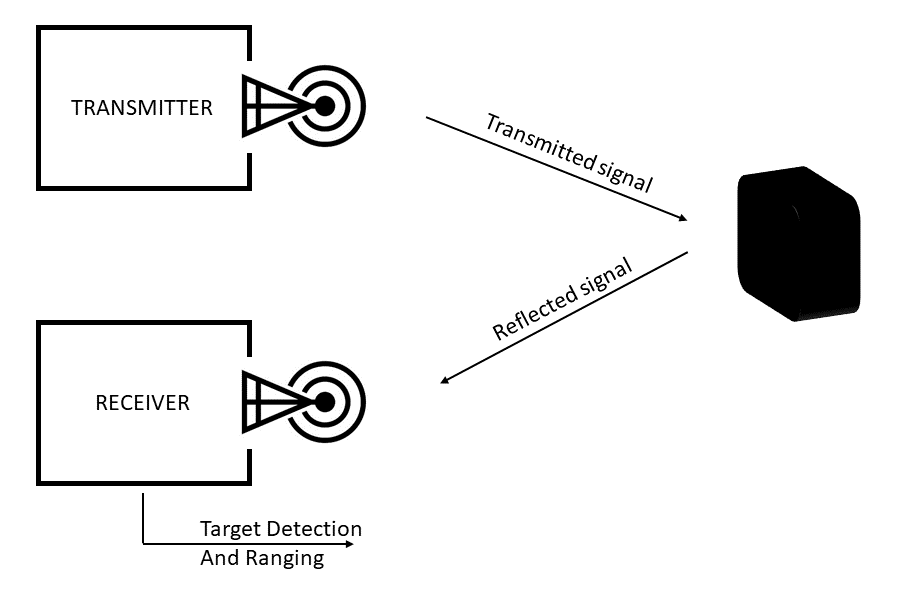
\includegraphics[width=0.70\textwidth]{Master's thesis/images/basic_block1.png} 
    \caption{The basic principle of RADAR.}
    \label{fig:basic_principle}
  \end{center}
\end{figure}

\subsection{Types of RADARs}

On a broad level, the RADARs can be divided into \begin{enumerate}
    \item \textbf{Pulse RADAR}
    
    In Pulse RADAR, the RADAR operates with Pulse signals. The RADAR sends the signals for a pulse of duration and then waits to receive the signals. The Pulse RADAR is further classified into Basic Pulse RADAR and Moving Target Indicator RADAR (MTI)
    \begin{enumerate}
    \item \textbf{Basic Pulse RADAR}
    
    It uses single antenna for both sending and receiving signals.  The antenna transmits signals after every clock pulse. This type of RADAR can only detect stationary objects.
    
    \item \textbf{Moving Target Indicator RADAR (MTI)}
    
    This type of RADAR uses pulse signals to compute even the non stationary objects. This uses Doppler effect to distinguish the non stationary object with stationary object.  
    
\end{enumerate}
    \item \textbf{Continuous Wave RADARs}
    
    On the other hand,  Continuous Wave RADARs sends continuous signals in order to detect objects. Both stationary and non-stationary objects can be detected using Continuous wave RADARs. Continuous wave RADARs are further divided into Unmodulated Continuous Wave RADAR  and Frequency Modulated Continuous Wave RADAR(FMCW).
    \begin{enumerate}

    \item \textbf{Unmodulated Continuous Wave RADAR}
   
    This type of RADAR detects non stationary objects using continuous wave signals. It is also called Continuous Wave Doppler RADAR. It is worth noticing that the frequency of the continuous signal remains unchanged over time.
    
    \item \textbf{Frequency Modulated Continuous Wave RADAR (FMCW)}
    
    This is the most advanced type of RADAR which can be used for detecting the both the stationary and non stationary objects.An FMCW RADAR requires two antennas- one for transmitting and the other one for receiving. The distance and velocity of the objects can be easily computed using Fourier transformations (FFT) of the received signals. More detailed explanation about FMCW is provided in the following section. 
\end{enumerate}
\end{enumerate} 







\subsection{Frequency Modulated Continuous Wave RADAR (FMCW)}

Continuous Wave Radar are popular because of low power consumption and simple radio architecture. Also,these type of Radars cancel out clutter noise by proper adjustment. The main advantages of the FMCW remains good range resolution, resistance to interception, simple solid-state transmitters. FMCW method performs the velocity and range measurement efficiently and therefore it is a good solution for lighting industry~\cite{arai2000life}~\cite{li2006experiment}.


FMCW generates a linearly increasing frequency signal viz., sawtooth or sinusoidal wave using a synthesizer. The generated signal is then transmitted using one or more antennas.
Each signal is called \textbf{chirp/sweep}. A chirp is a signal whose frequency increase linearly with time ~\cite{rao_2017}. A chirp can be characterized by the four features broadly-

\begin{itemize}
    \item start frequency which is generally called carrier frequency and denoted by \(f_{c}\),
    \item a chirp bandwidth(\(B\)), which is the difference between the maximum reachable frequency  \(f_{c} + B \)  and the carrier frequency \(f_{c}\).
    \item the sweep time(\(t_{p}\)), which is the duration for which an FMCW sends one chirp,
    \item The slope(\(k= B/t_{p}\)), of the chirp which is defined as rate at which the chirp ramps up. It is the ratio between the chirp bandwidth and the sweep time.
    
 \begin{figure}[ht]
  \begin{center}
    % below the size of the figure has been reduced for example
    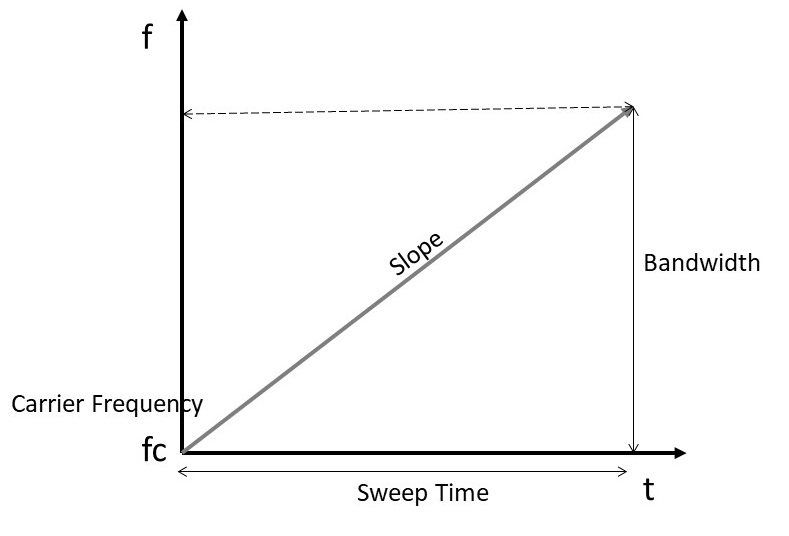
\includegraphics[width=0.60\textwidth]{Master's thesis/images/sweep.jpg} 
    \caption{A basic Chirp/Sweep signal}
    \label{fig:sweep}
  \end{center}
\end{figure}   
\end{itemize}

Therefore, the frequency of the signal \(f_{t}\) at any time \(t\), with carrier frequency \(f_{c}\) , amplitude \(A_{t}\), slope \(t\), is given by the following expression

\[f_{t}= A_{t}cos[2\pi(f_{c}t + \frac{k}{2}t^2)]\]

The transmitted signal TX is transmitted through the transmitter antenna. The TX signal strikes the surface of the object and gets reflected back. The receiver of the FMCW receives this reflected signal RX via its receiving antenna. RX signal is just the same TX signal but delayed.
To compute the range, velocity or phase of the object, the most important factor to measure is the \textbf{Baseband signal} with frequency IF known as \textbf{Intermediate Frequency (IF)}. The frequency of the Baseband signal is the difference of the instantaneous frequency of the TX-chirp and RX-chirp. It is to be noted that for a stationary object, irrespective of when the  chirp was transmitted, this IF signal will remain same, as this IF signal is proportional to the delay time which is proportional to the distance of the object from Radar. Figure ~\ref{fig:IF} explains the IF signal in the mathematical way. 

\begin{figure}[!tbp]
  \centering
  \begin{minipage}[b]{0.4\textwidth}
    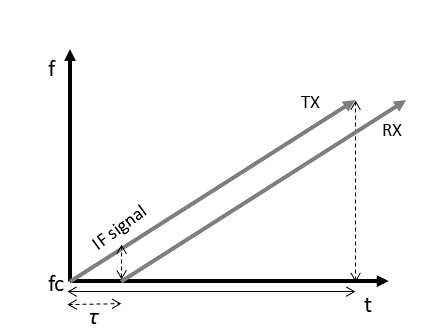
\includegraphics[width=\textwidth]{Master's thesis/images/IFSignal.png}
    \caption{IF Signal}
    \label{fig:IF}
  \end{minipage}
  \hfill
  \begin{minipage}[b]{0.55\textwidth}
    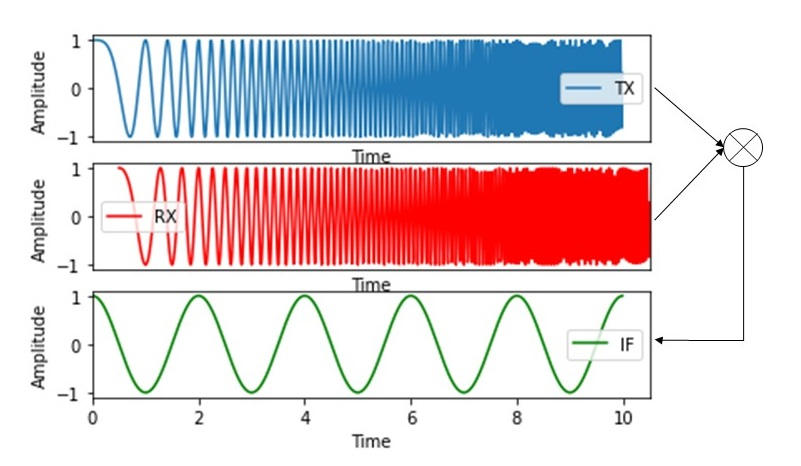
\includegraphics[width=\textwidth]{Master's thesis/images/mixer.jpg}
    \caption{IF signal from TX and RX}
    \label{fig:Mixer}
  \end{minipage}
\end{figure}

 \begin{figure}[ht]
  \begin{center}
    % below the size of the figure has been reduced for example
    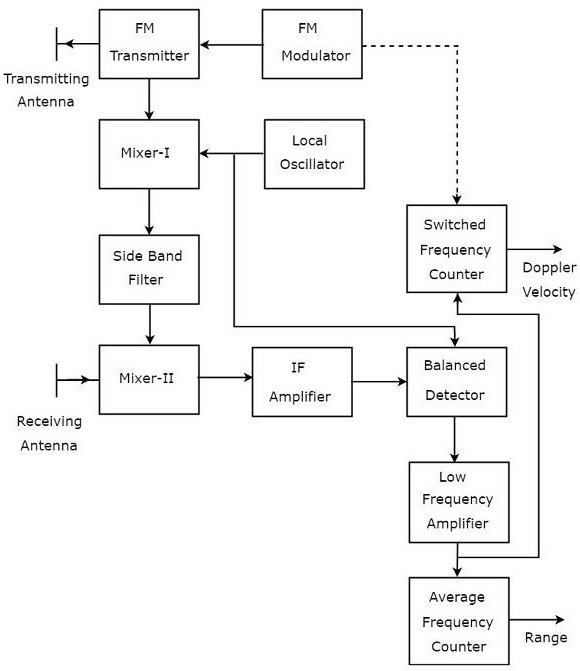
\includegraphics[width=0.650\textwidth]{Master's thesis/images/fmcw_working.jpg} 
    \caption{Block Diagram for FMCW}
    \caption*{\textit{Source:} Radar Systems - FMCW Radar~\cite{tutorialspoint}.}
    \label{fig:fmcw}
  \end{center}
\end{figure}   

Figure ~\ref{fig:fmcw} explains in detail on how this Baseband signal is produced. 
The \textbf{Frequency Modulator} produces a modulated frequency signal TX which is transmitted using \textbf{Transmitter}. The \textbf{Local Oscillator} produces a signal having Radio Frequency \(f_{rf}\). The output of the Local Oscillator is then feeded to a mixer along with the output of the Transmitter. The \textbf{Mixer} computes then sum and the difference of the Transmitted frequency and the RF signal from Local Oscillator. A low pass filter then only allows the lower frequency to be passed i.e. only the difference of the Transmitter and the RF signal \(f_o(t) - f_{rf}\) is allowed. ~\cite{tutorialspoint}. 

Another \textbf{Mixer}, is feeded the received signal from the receiving antenna \(f_r\) and the output of the low pass filter. It is worth mentioning that the received signal RX is just a delayed version of the transmitted signal TX. It then computes the sum and the difference of these signals again, i.e. \(f_r\) + \(f_o(t) - f_{rf}\), \(f_r\) - (\(f_o(t) - f_{rf}\))~\cite{tutorialspoint}. An \textbf{Amplifier} amplifies the differenced output of the Mixer, i.e. only \(f_r\) - \(f_o(t) + f_{rf}\) is amplified. The \textbf{Balance Detector} which is connected to both the Amplifier and the Local Oscillator computes the difference of the both input signals, hence generating a signal of frequency \(f_r - f_o(t)\). 
This output is then inputted to \textbf{Low Frequency Amplifier} which amplifies the input frequency. This resultant signal is then called the Baseband signal ~\cite{tutorialspoint}. 


In order to understand the functionality of FMCW in better detail, we will divide the topic into 3 parts.
\begin{itemize}
    \item Part 1: Evaluation of the range of the target object.
    \item Part 2: Evaluation of velocity of the target object.
    \item Part 3: Evaluation of phase of the target object.
\end{itemize}

\subsection{Signal Processing for FMCW}
The Baseband signal is constructed by the Radar when an object reflects the signals. However in a real scenario, there are multiple objects in the scene resulting in multiple Baseband signals. Therefore Radar receives combination of these Baseband signals. To differentiate different objects, Radar should be able to differentiate between different signals. To do so, Radar uses Fourier Transformations. A brief summary of Fourier Transformations is provided in the following subsection.


\subsubsection{Fourier Transformation} \label{sec:FT}
According to ~\cite{FT}
\say{Fourier transform (FT) is a mathematical transform that decomposes functions depending on space or time into functions depending on spatial or temporal frequency.}
Specific to FMCW, Fourier Transform is used to convert a time domain signal into the frequency domain. 
Consider a frequency signal in the form -  
\begin{equation}\label{eq:eq1}
A_{t}= ASin[2\pi ft + \phi]
\end{equation}
Let's suppose A =2, t= 1sec, \(\phi\) = 0 and f = 4.
\\
Therefore, the eq ~\ref{eq:eq1} becomes
\begin{equation}
A_{t}= 2Sin[8\pi]    
\end{equation}

The Fourier Transformation of this signal, returns a frequency-amplitude domain signal, with a peak at \textbf{4} as the frequency of the signal was 4.

 \begin{figure}[ht]
  \begin{center}
    % below the size of the figure has been reduced for example
    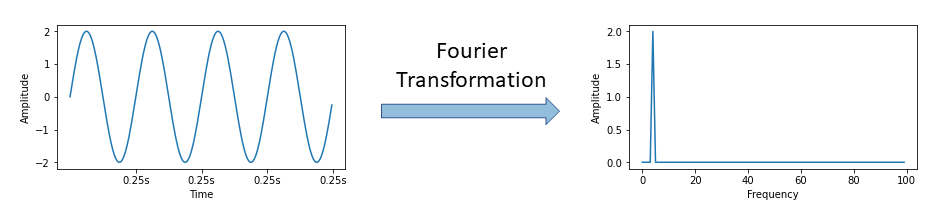
\includegraphics[width=1\textwidth, height = 3.5cm ]{Master's thesis/images/fft.png} 
    \caption{Fourier Transformation of a constant frequency signal}
    \label{fig:fft}
  \end{center}
\end{figure}  

However, in a real time scenario, signals are not continuous, rather discrete. Therefore for discrete signals, Discrete Fourier Transform (DFT) is commonly used. The resolution limit is determined by the number of input samples.
The output of the DFT has the same size as input. For a device like Radar where the frequency of the signal is usually in GHz, the sampling index is huge, therefore the number of outputs of DFT will be huge. Increasing the number of inputs, increased the computation power by $O[N^2]$.
\\

Therefore, to make the computations less complex, the number of samples are chosen as a power of $2^N$ which enables to use Fast Fourier Transform (FFT) instead of DFT. The complexity of FFT is $O[NlogN]$ instead of $O[N^2]$. FFT can be used either by increasing the sampling rate or by appending zeros at the end before performing FFT. Zero padding makes the resolution between two consecutive bins easier.

It is worth mentioning that the resolution of the FFT increases with the length of the observation period. In general, an observation window if T can separate frequency components that are separated by more than $\frac{1}{T}$ Hz~\cite{rao_2017}.
%windowing%


\subsubsection{Range Evaluation for Stationary targets}\label{sec:rangeEval}

Consider an object as distance $d$ from the FMCW Radar. From ~\ref{fig:IF}, we can clearly say that the frequency of the IF signal is 
\begin{equation}\label{eq:range}
    f_{\tau}= k\tau
\end{equation}
where k is the slope of the chirp, $\tau$ is the delay in the RX signal.
But 
\begin{equation}
    Time = Distance*Speed
\end{equation}
Therefore, substituting Distance = 2d ( To and fro distance covered by the signal from Radar) and Speed = c (speed of light) into eq ~\ref{eq:range}, we get:
\begin{equation}\label{eq:range_eq}
f_{\tau}= k\frac{2d}{c}   
\end{equation}

Eq ~\ref{eq:range_eq} indicates the Intermediate frequency of the Baseband signal obtained from an object placed at a distance d.
\\


In a real scenario, an FMCW receives a signal which is a combination of different Intermediate Frequencies. These IF signals are produced by objects placed at different ranges. From Eq~\ref{eq:range_eq}, it is evident that these IF signals are proportional to the distance d at which the object is placed.
This is where Fourier Transformations discussed in section ~\ref{sec:FT} comes into picture.

To calculate the range of different objects present in the view, the output received by the FMCW Receiver is transformed using FFT. This result is called \textbf{Range FFT} of the received signal RX.

For instance, let's imagine the receiver receives the composite signal as shown in the Fig \ref{fig:comp_fft}. The signal is formed by addition of two different IF signals with frequencies of 4 Hz and 6 Hz, and the amplitude of 2 m and 3 m.
The frequencies and the amplitude of these composite signals can be easily obtained by using FFT on this signal. The plot beneath the composite signals indicates the FFT output on the composite signal.
Therefore, in a real time scenario to obtain a range estimation of all the objects in the frame, it is important to use Range FFT.
 \begin{figure}[ht]
  \begin{center}
    % below the size of the figure has been reduced for example
    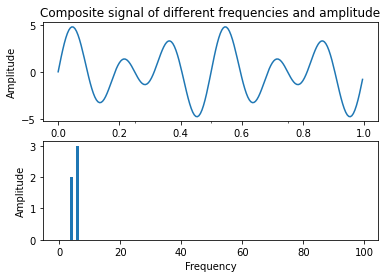
\includegraphics[width=0.6\textwidth]{Master's thesis/images/comp_fft.png} 
    \caption{Fourier Transformation of a composite signal}
    \label{fig:comp_fft}
  \end{center}
\end{figure}  

\textbf{Range Resolution} is defined as the minimum distance that should be there in between two objects to differentiate them for FMCW. As previously explained, in order to differentiate two objects, the frequency difference should be at least 1/T i.e., 
\begin{equation}\label{eq:fgtt}
 \Delta f > \frac{1}{T}  
\end{equation}Consider two objects, placed at a distance of $d_{1}$ and $d_{2}$, from eq~\ref{eq:range_eq}, their respective IF frequencies are given by
 \begin{equation}
   f_{\tau1}= k\frac{2d_{1}}{c}
 \end{equation} 
 
 and
  \begin{equation}
   f_{\tau2}= k\frac{2d_{2}}{c}
 \end{equation} 
 
 Therefore, 
 \begin{equation}\label{eq:deltaf}
     \Delta f = k\frac{2\Delta d}{c}
 \end{equation}
Substituting Eq~\ref{eq:deltaf} in Eq ~\ref{eq:fgtt} and T with the observation period $T_{c}$, we get,
\begin{equation}
  k\frac{2\Delta d}{c} > \frac{1}{T_{c}}  \implies \Delta d > \frac{c}{2kT_{c}} \implies \Delta d > \frac{c}{2B}  
\end{equation}
where $B$ is the Bandwidth of the chip and is equal to $kT_{c}$.

Hence, the Range Resolution ($d_{res}$), depends only on the speed of the light and Bandwidth of the chirp~\cite{rao_2017}, $\therefore$ 

\begin{equation}
   d_{res} = \frac{c}{2B} 
\end{equation}

\textbf{Maximum Range} of the Radar is defined as the distance beyond which FMCW fails to operate. From Eq. ~\ref{eq:range_eq}, substituting $d$ with $d_{max}$, we get \(f_{IF_max} = \frac{k2d_{max}}{c}\) . Replacing $f_{IF_max}$ with $F_{s}$,where $F_{s}$ is the maximum sampling rate of Radar, we have,
\begin{equation}
    d_{max}= \frac{F_{s}c}{2k}
\end{equation}

This means we an increase or decrease the maximum field of view range by changing either maximum sampling rate or the bandwidth.
\begin{itemize}
    \item Keeping Maximum Sampling rate constant $F_{s}$, the Maximum Range of the Radar can be manipulated by changing the Bandwidth.
    \item Similarly,  Keeping Bandwidth constant, the Maximum Range of the Radar can be manipulated by changing the Maximum Sampling Rate $F_{s}$.
\end{itemize}



\subsubsection{Velocity Evaluation for Moving targets}
According to section~\ref{sec:rangeEval}, to separate different objects in the view, Range FFT is applied on the received RX signal. However the question to ask here is "\textit{How can the two objects placed at same radial distance from FMCW can be separated?}"~\cite{rao_2017}. The FFT of the two objects placed at same distance will give peak bins at the same frequency. However doing further signal, this problem can be resolved using the velocities of these object which are at same distance. It is to be noted that these objects can be differentiated if the velocities of these objects are different.

To solve this problem, Fourier Transformation comes into the picture. However instead of doing Range FFT, \textbf{Doppler FFT} is used.

Let's go a step further to what is explained in sec ~\ref{sec:FT}. Note that using Euler's formula, any sinusoidal signal in rectangular form can be expressed in the form of complex exponential signal. A Euler's formula is expressed as \(Ae^{j\theta}\), where $A$ is the amplitude of the signal and $\theta$ is the initial phase of the signal. The Fourier transformation of the signals produces a complex signal, i.e, an amplitude value as well as the phaser. 
In the Fig ~\ref{fig:euler}, waves and their corresponding Euler's representations are shown.

 \begin{figure}[ht]
  \begin{center}
    % below the size of the figure has been reduced for example
    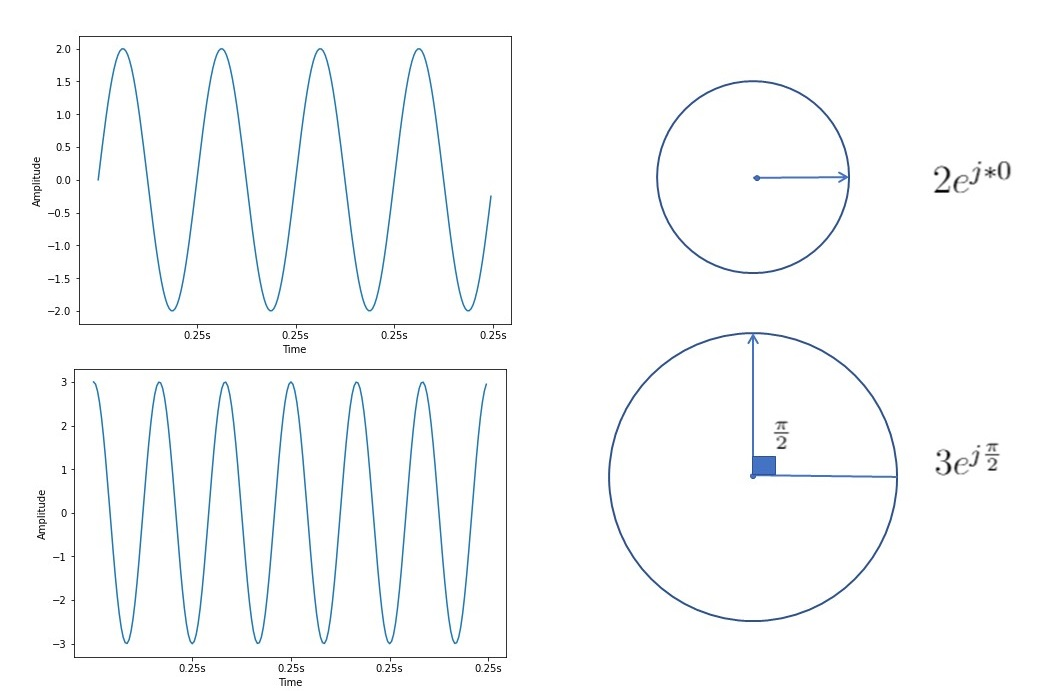
\includegraphics[width=0.8\textwidth]{Master's thesis/images/euler.jpg} 
    \caption{Wave and its Euler representation}
    \label{fig:euler}
  \end{center}
\end{figure}  

Now, consider the Fig ~\ref{fig:Mixer}, what happens if the target object moves by a distance of $\Delta d$. It can be surely said that the frequency of the Baseband signal i.e, Intermediate Frequency will be change by $\frac{2\Delta d}{c}$. This value is close to 0, since $\Delta d$ is very small. However, the initial phase of the IF signal will definitely change, despite the fact that the intermediate frequency is same. Change in $\Delta d$ makes $\Delta\tau$, round trip delay.
Phase $\theta$ of a wave at any time t, can be represented as-
 \begin{equation}
     \theta= 2\pi ft
 \end{equation}
Therefore change in theta with change in time $\Delta t$ is-
 \begin{equation}
     \Delta\theta= 2\pi f\Delta t
 \end{equation}
 For the purpose of simplicity, we represent change in phase i.e, $\delta \theta$ with $\omega$. It is known that, $\Delta t= \frac{2\Delta d}{c}$ and $f= \frac{c}{\lambda},  \therefore$ putting everything together - 
 \begin{equation}\label{eq:theta}
     \omega= \frac{4\pi \Delta d}{\lambda}
 \end{equation} 

This is the change in phase of the IF signal, when an object moves by distance 
\begin{equation}\label{eq:eq1}
A_{t}= ASin[2\pi \frac{k2d}{c}t + \frac{4\pi \Delta d}{\lambda}]
\end{equation}
The phase of the IF signal is very sensitive to to small change in object range ~\cite{rao_2017}.

 \begin{figure}[ht]
  \begin{center}
    % below the size of the figure has been reduced for example
    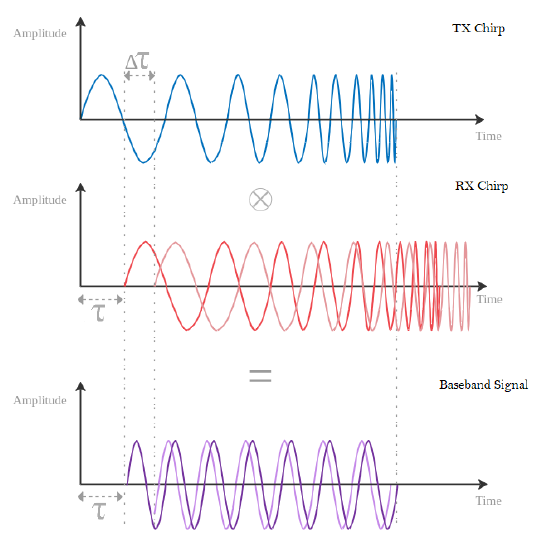
\includegraphics[width=0.6\textwidth]{Master's thesis/images/delay_sweeps.PNG} 
     
    \caption{Two consecutive chirps giving rise to a phase difference}
    \caption*{\textit{Source:} Nilsson, J., Hassbring, L. (2020). Machine Learning for FMCW Radar Interference Mitigation~\cite{nilsson2020machine}.}
    

    \label{fig:delay}
  \end{center}
\end{figure}  

To calculate the velocity of the object, two chirps are transmitted separated by time interval of $T_{c}$.
It is known that $d= vT$ (v is velocity of the target object), From Eq. ~\ref{eq:theta}, substituting $\Delta d$, we get -
\begin{equation}
    \omega= \frac{4\pi v \Delta t}{\lambda}
\end{equation}
Substituting $\Delta t$ with $T_{c}$, which is the time between two consecutive sweeps and reordering, we get-

\begin{equation}
    v= \frac{\lambda \omega}{4\pi T_{c}}
\end{equation}
Therefore, in summary, it can be said that the phase difference obtained from the Fourier transformation of two consecutive chirps, can help in determining the velocity of that object. 

The phase shift between consecutive chirps is the same for any two chirps. This phase shift can be easily calculated by performing FFT on the Range FFT from each chirp. This is called Doppler FFT. The whole process is the called Range-Doppler FFT, i.e, first performing Range FFT on the signals to evaluate the Range and then performing another Doppler FFT on consecutive chirps to obtain the velocities of these objects and then to differentiate them. 
The Range Doppler FFT is done with the help of matrix, with the dimensions N x M where M is the number of chirps and N is the number of samples in each chirp.

A proper visualization of the Range-Doppler FFT process can be seen in Figure ~\ref{fig:range-doppler-FFT}. Every IF signal/Baseband signal have its own phase. Every baseband signal is inserted row wise in a matrix. Every row undergoes a Range FFT operation for Range estimation. This is done in parallel as soon as the FMCW received the RX signals. The result is peak in some columns of the matrix. Once the number of received signals are enough, column wise FFTs are performed for a radial velocity estimation.
 \begin{figure}[ht]
  \begin{center}
    % below the size of the figure has been reduced for example
    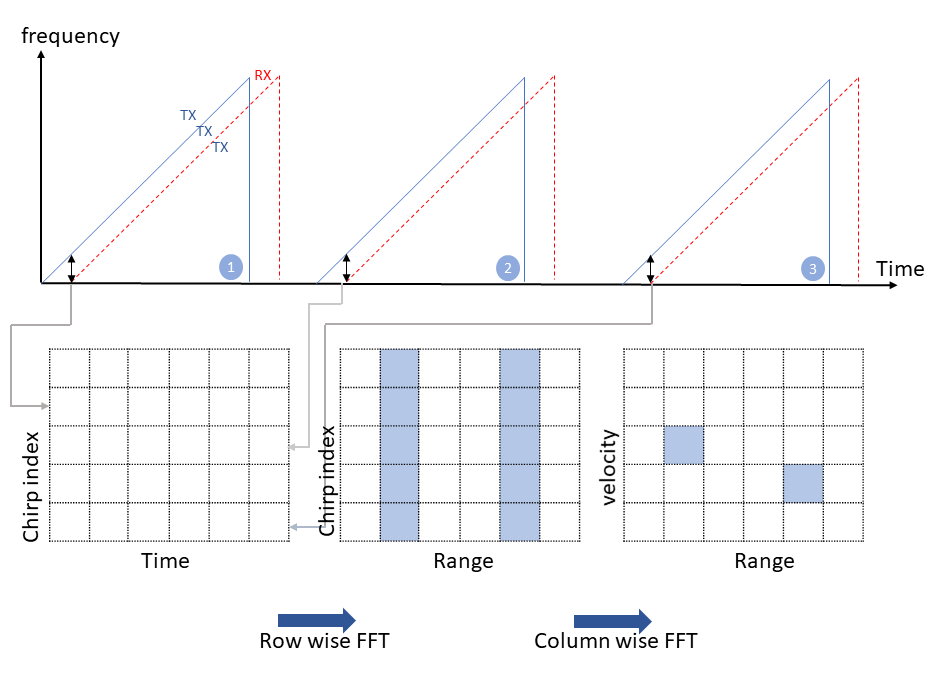
\includegraphics[width=0.7\textwidth]{Master's thesis/images/range_doppler1.png}
    \caption{Range-doppler-FFT}
    \label{fig:range-doppler-FFT}
  \end{center}
\end{figure}  



This results in peaks in different cells of the matrix. These cells corresponds to different objects at different locations from FMCW and moving at a different radial velocity to/from FMCW. The Doppler-FFT change the Range x Chirp index dimension to Range x Velocity. Also, frequency is changed from the range from [0, $2\pi$] to [-$\pi$,$\pi$] in the normalized frequency domain. This makes sure that even the negative velocities are captured.

Therefore in summary, it can be said that for the object at different ranges or the objects at different ranges can be easily detected using Range-Doppler FFT.

\subsubsection{Phase Evaluation for moving targets}

In the previous subsection, the complete process about Range-Doppler FFT was explained. However, now one most case rises up, where the Range-Doppler FFT fails completely. Consider a case where two objects at same radial distance are moving to/from the FMCW at the same radial velocity. The Range-Doppler FFT will give rise to one bin for two different object. So this situation forces us to ask the question
\textit{"How can the two objects placed at same radial distance and moving with same radial velocity from FMCW can be  separated?"}

A very simple answer is to give two eyes to the FMCW. The main advantage of humans having two eyes is to interpret the world in 3D, i.e, humans can perceive the depth of the objects in field of view because eyes are located at different points. So using this analogy, if we use multiple receiving antennas for the FMCW, it will help us solving the problem in question.

An FMCW measures Angle of Arrival(AoA) to resolve this problem. Angle estimation will require a minimum of 2 receiver antennas. Assuming the receiver antennas are placed in close proximity, there ratio of the radial distance from one antenna with other will be close to 1. This means, even if the two antennas in consideration have some Range FFT (as they are almost at same radial distance from the object), there will be a phase change involved. Eq. ~\ref{eq:theta}, shows that an object which made a small change in distance $\Delta d$ in two consecutive sweeps give rise to a phase difference $\Delta \theta$ or $\omega$.
\[\omega= \frac{4\pi \Delta d}{\lambda}\]
Using the same mathematical notation, it can be said that the phase difference between the two antennas will be
\begin{equation}\label{eq:AoA}
\omega= \frac{2\pi \Delta d}{\lambda}    
\end{equation}
Here is the eq.~\ref{eq:AoA}, the equation has a factor of 2 instead of 4 in eq.~\ref{eq:theta}. The difference can be understood by mere intuition. When an object moves by some distance $\Delta d$, the phase difference will brought out by the two and fro signal. Here , in contrast, the phase difference is brought by the distance between the two receiving antennas. This is the reason the eq. has been divided by 2 ~\cite{rao_2017}.
 \begin{figure}[ht]
  \begin{center}
    % below the size of the figure has been reduced for example
    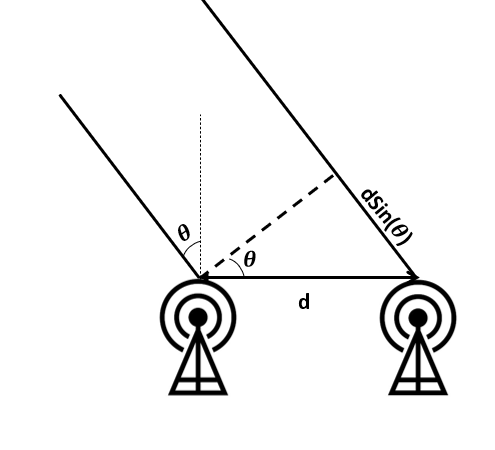
\includegraphics[width=0.3\textwidth]{Master's thesis/images/AoA.PNG} 
    \caption{Angle of arrival in case of two receiver antennas}
    \label{fig:AoA}
  \end{center}
\end{figure}  
Using the geometry of Fig ~\ref{fig:AoA} and using eq.~\ref{eq:AoA}, it can be derived that-
\[\omega= \frac{2\pi dsin(\theta)}{\lambda}\]
Hence, $\theta$ which is the AoA can be derived as-
\begin{equation}
    \theta= sin^{-1}(\frac{\lambda\omega}{2\pi d})
\end{equation}
It is worth mentioning that the maximum phase difference can be more than $\pi$, For phase difference more than $\pi$,it will be impossible to say of the phase difference was actually $\theta$ or $\theta-\pi$.

Now consider the \textbf{figure},it is pretty much evident that the two objects at same radial distance will result in same peaks in the Range-Doppler FFT, however multiple antennas give rise to a phase difference.




If another FFT is applied on these phase differences, this give rise to an FFT sequence which is called \textbf{angle-FFT}. Angle FFT helps in resolving such two objects.


%\subsubsection{Micro Doppler}


\subsection{RADAR Specifications}
The RADAR used in this thesis has a carrier frequency of 24 Ghz. The Bandwidth of the frequency is 250 MHz and the sweep time is 1 ms.

Specify about antennas and receivers
\begin{figure}[ht]
  \begin{center}
    % below the size of the figure has been reduced for example
    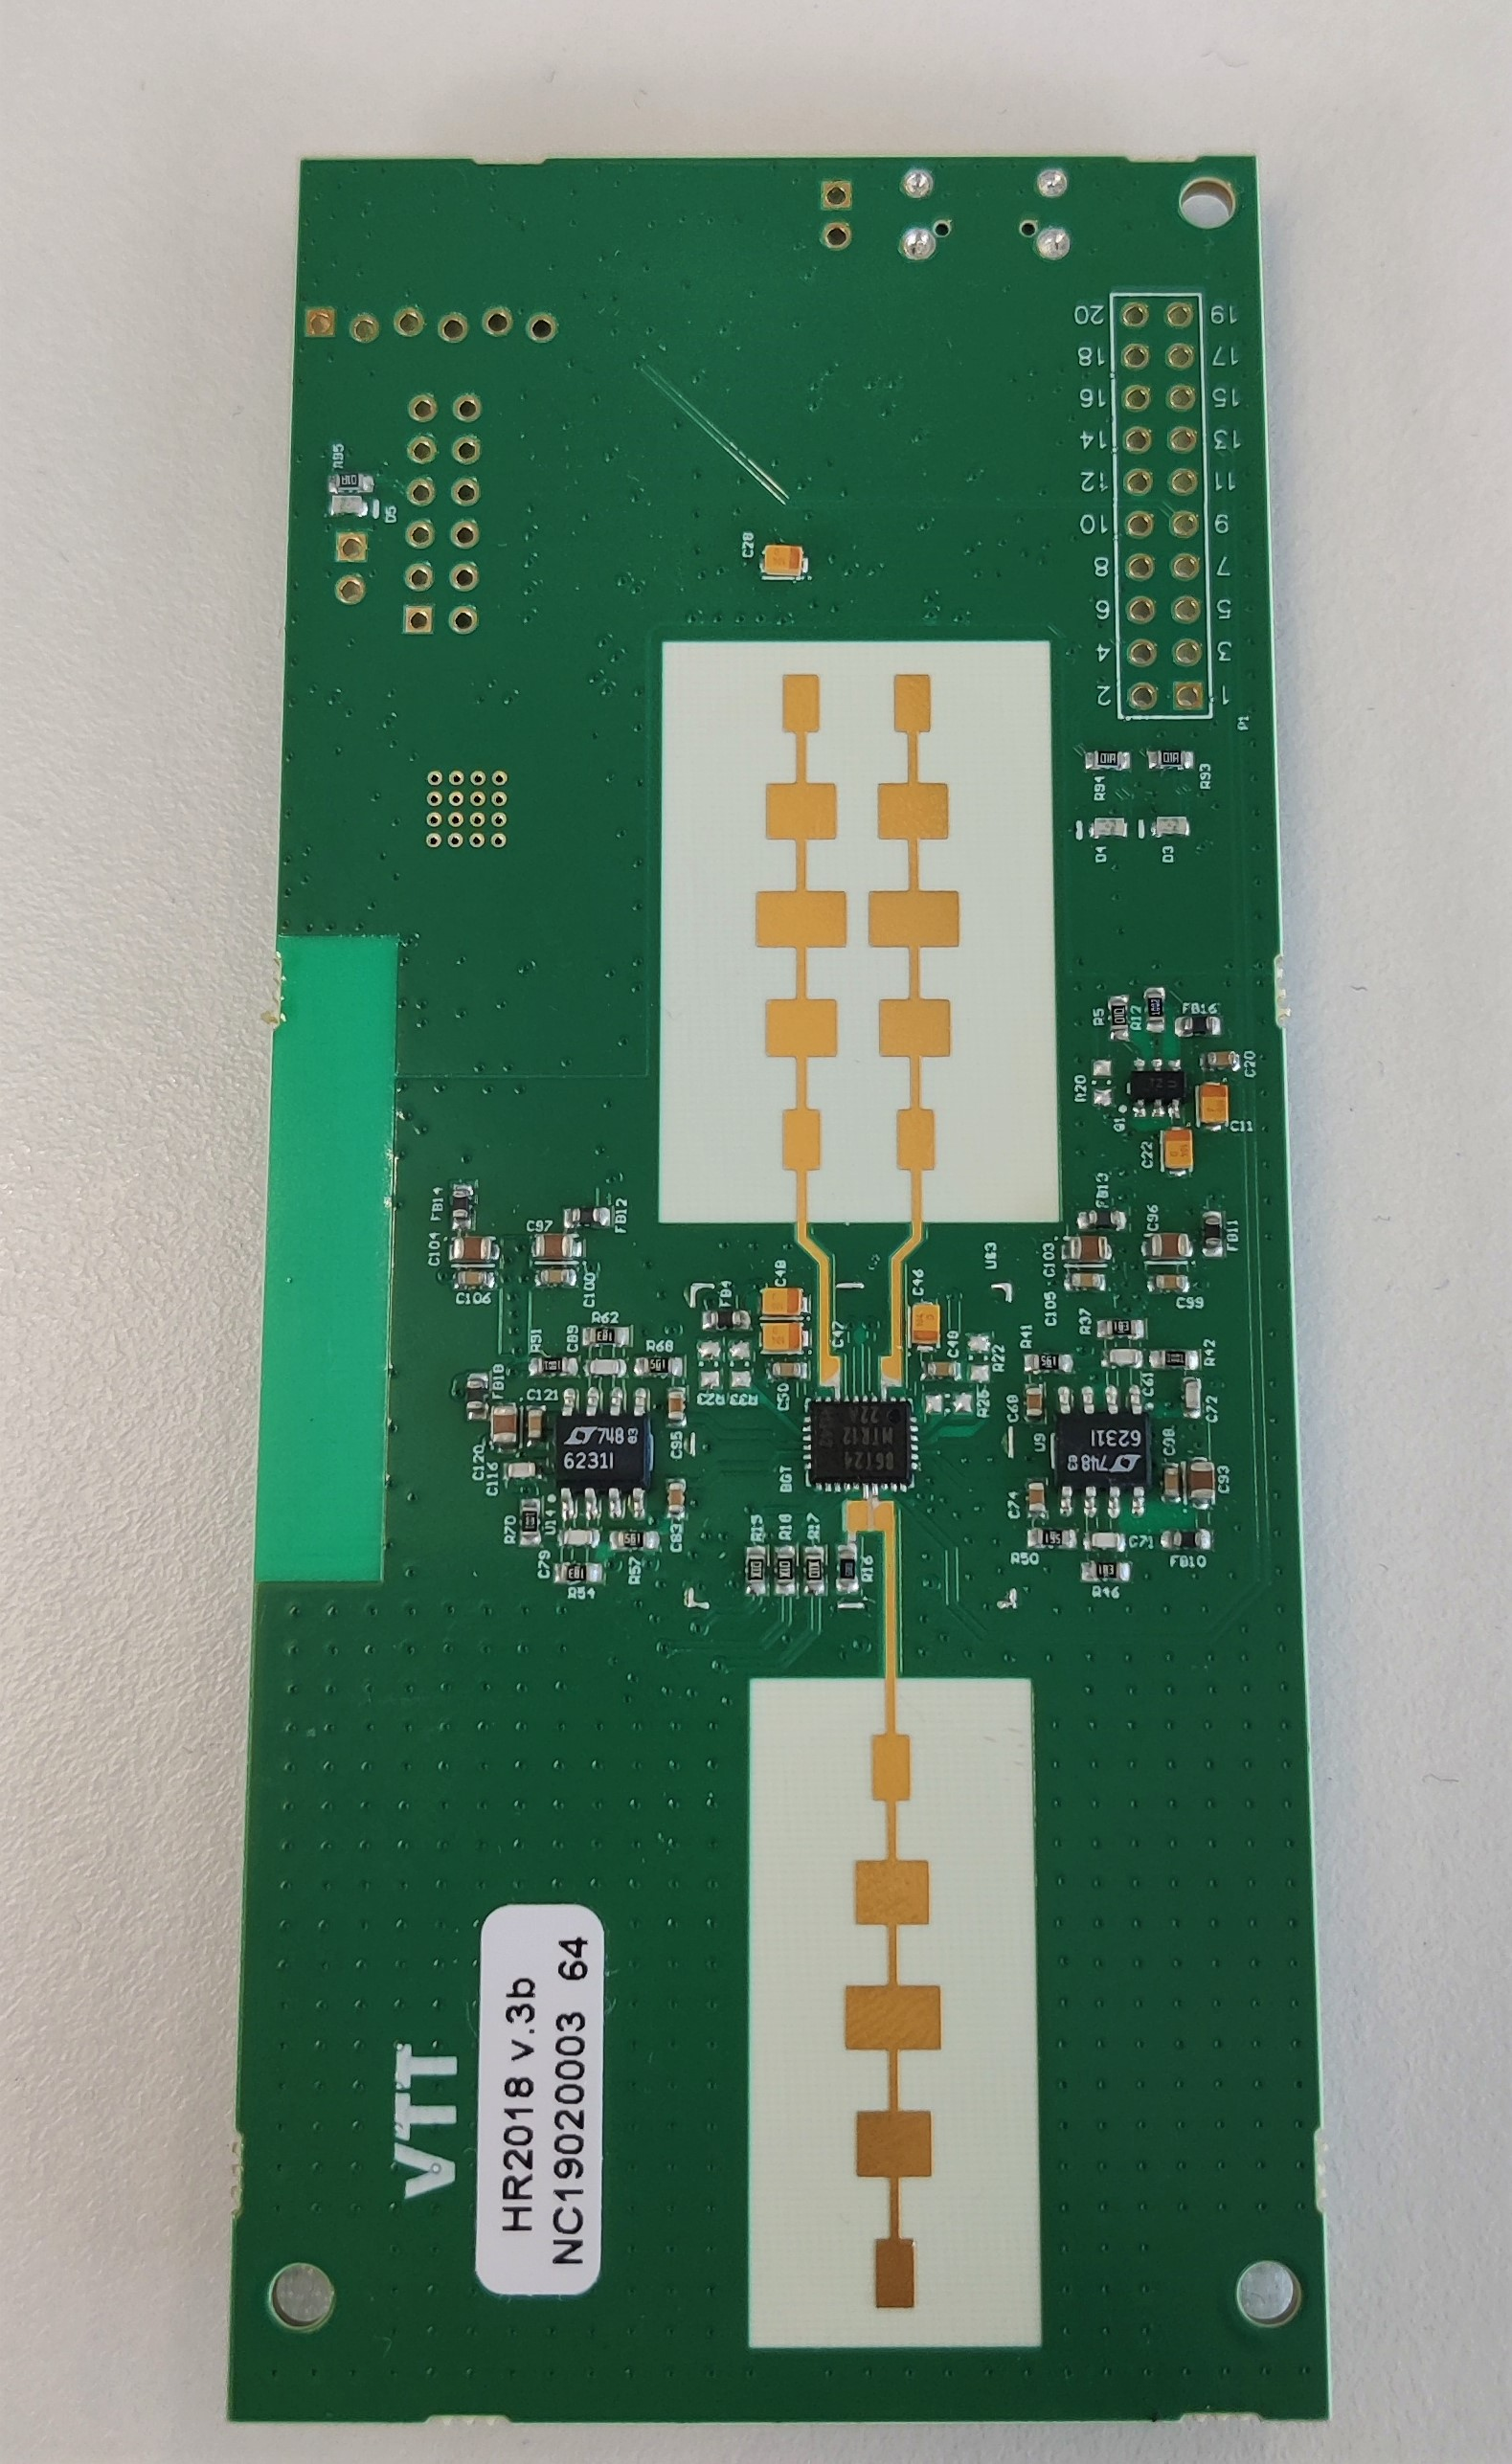
\includegraphics[scale = 0.08]{Master's thesis/images/Radar_internal.jpg} 
    \caption{Internal details of the RADAR}
    \label{fig:AoA}
  \end{center}
\end{figure}  




\begin{center}
\begin{tabular}{ |c|c|c| }
\hline
 S.No. & Specification & Value \\ 
 \hline
1 &	Carrier Frequency	& 24 Ghz \\
2	& Bandwidth of 1 sweep	& 250 MHz\\
3 &	Sweep Time	& 1 ms\\
4 &	Min sweep interval	& ~16.7 ms\\
5 &	Centre Angle & 210$^{\circ}$  \\
6 &	Max view distance &	14 m \\
 \hline
\end{tabular}
\end{center}

\section{Artificial Intelligence}
Artificial intelligence (AI) is intelligence demonstrated by machines, unlike the natural intelligence displayed by humans and animals, which involves consciousness and emotionality. 'Strong' AI is usually labelled as artificial general intelligence (AGI) while attempts to emulate 'natural' intelligence have been called artificial biological intelligence (ABI) ~\cite{poole1998computational} .
There are numerous ways to define Artificial Intelligence (AI) as there are many controversial discussions about the definition of human intelligence. On a broader level, the AI is an umbrella term for any hardware or software that enables a machine to mimic human intelligence. AI should be adaptive and, in many cases, autonomous as well ~\cite{touger2020}.
\subsection{Machine Learning}

Machine Learning (ML) is a subset of AI. It is the study of computer algorithms that improve automatically through experience and by the use of data ~\cite{mitchell1997machine}. With the help of Mathematics, Statistics and Probability, the machines can learn from the data and then can make decision on the new unseen data. ML allows to automatically extract relevant information from data applying it to analyze new data.
There are several machine learning methods. Different methods can be tested to determine the best option for a certain problem. The ML algorithms are classified into supervised , unsupervised learning and Reinforcement Learning algorithms.
\newline

\noindent \textbf{Supervised Learning}
\newline

\noindent In Supervised learning, the goal is to estimate the unknown model that maps known inputs to known outputs. The data-set, in that case, has defined targets or labels that are pre-determined. The problem can be classification, Regression or Probability estimation. Training set can be defined in the form \( D = {<x,t>} => t = f(x)  \) where D is the dataset, x is the feature vector, t is the target variable. Numerous algorithms are used for supervised learning like Support Vector Machines, Decision Tree, K-Nearest Neighbors, Naive Bayes etc. 
\newline

\noindent \textbf{Unsupervised Learning}
\newline

\noindent On the contrary, In Unsupervised learning, the goal is learning a more efficient representation of a set of unknown inputs. Here the expected targets are not
provided to the algorithm. Therefore, the algorithm has to learn some patterns in the data without any supervision or prior knowledge of what the data-set might be about.  Training set can be defined in the form \( D = {x} => ? = f(x) \) where D is the dataset, x is the feature vector, ? is the unknown representation. The most common problems in unsupervised learning includes Clustering and Compression. Numerous algorithms are used for unsupervised learning like K-Means, Self organizing maps, Principal Component Analysis etc.
\newline

\noindent \textbf{Reinforcement Learning}
\newline

\noindent Reinforcement learning is an area of Machine Learning which is about deciding the best suitable action to maximize reward in a particular situation. It is used in many software and machines to find the best possible behavior or path it should take in a specific situation. Reinforcement learning differs from the supervised learning as in the later, the training data has the correct label with it so the model is trained with the correct answer itself whereas in the former, there is no answer but the reinforcement agent decides what to do to perform the given task. In the absence of a training dataset, it is bound to learn from its experience \cite{geeksforgeeks_2020}.




The main challenge with Machine Learning is that it is supposed to perform efficiently on new, unseen data. In order to verify of the Machine Learning models performs well on the new data, usually the dataset is divided into training and test set. The model is trained on training data. No where in the training process, the test data set is involved. A good model should give high performance on test data set along with the train data set. This feature is called generalization.The generalization error i.e test error must be minimized. The trained model’s performance is tested with the
test set to measure generalization error. If there is high performance on train dataset and low performance on test dataset, the model is said to have over fitted the train set, or simply it has just learned the train set.

Some of the factors that determine the performance of the ML include the training error, test error and the gap between them. More detailed information about train set and test set performance is provided in the next section.

\subsection{Deep Learning}
Machine Learning tasks can be solved by designing the right set of features to extract. One can use the domain knowledge to design features that are robust. While the domain knowledge works perfectly fine for most the cases like the cases where features can be numerically or quantitatively explained, however problem arises for situation like images, videos or text. For such tasks, it is difficult to known what features should be extracted. It maybe possible to extract the features in image context with the algorithms that considers intensity and change in intensity with respect to pixels. However most of the times, these features are not perfect and eventually forces the researcher to reiterate the feature extraction phase.

These problems can be solved with Representation learning, i.e, we use Machine Learning not only to predict the mapping of the representation, but also the representation itself.Deep learning is a subset of Machine Learning based on artificial neural networks which learns the representations.
Deep learning solves the central problem in representation learning by introducing representations that are expressed in terms of other, simpler representations. Deep learning enables the computer to build complex concepts out of simpler concepts ~\cite{Goodfellow-et-al-2016}.  

Deep Neural Networks is a supervised learning approach of a deep network of processors called neurons.
A neuron originally is a biological term for a fundamental unit of the brain. The
neuron is designed to pass electrochemical signals to the other neurons and to other parts
of the brain ~\cite{Goodfellow-et-al-2016}. The architecture of the artificial neural network is inspired by the brain's neural networks.
The neural network processors receive and transmit signals between each other. The
neurons store and process information in the connections between the neurons which are
called weights. The weights are multipliers on the inputs of the neuron.
\newline

\noindent \textbf{Neural Networks}
\newline

\noindent The Deep Neural Networks are composed of layers. Each layer further is composed of several neurons. The input layer or the first layer of the network get their inputs directly from the data. For
example, in the case of an image, the input layer consists of all the pixels values of the image. The rest of the layers of the network (hidden layers) use the previous layer's outputs as their input and feed their produced output to the proceeding layer. The final layer is called the output layer which is used for delivering the output of the whole neural network.
The depth of the deep learning system enables the computer to learn a hierarchical program. Each layer has some instructions
that are executed in parallel. Instructions in different layers are executed sequentially
in the order of the layers. There is state information that is similar to the pointer in a
traditional computer program. The state information is stored in the representation of the neural network



\noindent \textbf{Training Neural Networks}

\noindent\textbf{Regularization}

\noindent \textbf{Hyper-parameter Tuning}

\noindent \textbf{Feedforward Neural Networks}

\noindent \textbf{Convolutional Neural Networks}

\noindent \textbf{Structure of a Convolutional Layer}

\noindent \textbf{Parameters of a Convolutional Layer}



%\section{Lighting Industry}
%\section{Machine Learning Literature Review}






\chapter{Methodology and Data Gathering}
\label{chapter:methodology}
This thesis will be focused mainly on Classification problem of the "human presence" i.e. if the human is present or not. This will be a Supervised Learning problem where the features will be mapped to the classes/labels.
For this thesis, we are using VTT built 25 GHz RADAR.The methodology includes Data collection, Data cleaning, Model Building and Model deployment. Here is a flow, how the process will be conducted in the upcoming months.


\begin{figure}[ht]
  \begin{center}
    % below the size of the figure has been reduced for example
    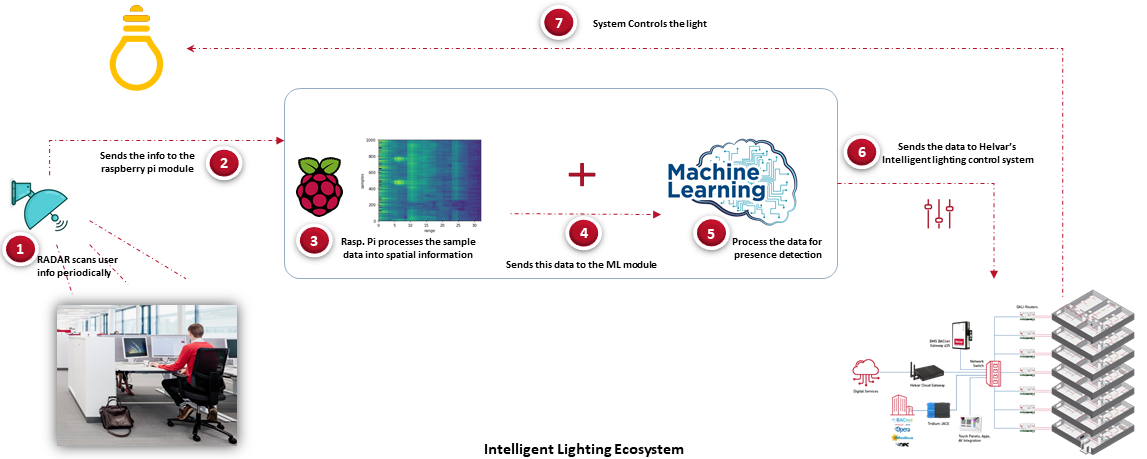
\includegraphics[width=1\textwidth]{Master's thesis/images/thesis_presentation.png} 
    \caption{Overall Process}
    \label{fig:basic_principle}
  \end{center}
\end{figure}


\begin{enumerate}
    \item RADAR box provides Analog to Digital converted signal. The data from these signals are collected over multiple hours at multiple locations.
    %However, this information is not sufficient to distinguish between human presence or absence. Therefore, in order to detect human presence i.e. to collect the labels for the data, we will be using RGB camera for the purpose of creating ground truth. RADAR data will be mapped with RGB presence detection based on each time frame.
    \item The data obtained will be feature engineered using multiple techniques.
    \item The idea is to engineer the received RADAR signal of every time frame (say 1 sec) to a 2-D map and then treating this 2-D map as an image or set of features.
    \item Deep Neural Networks or other Machine Learning techniques will be applied on this already processed data.
    \item For the purpose of training, we will leverage the cloud resources by AWS.
    \item The last step is to deploy these models on the edge devices.
\end{enumerate}

The ultimate objective is to create a more sustainable lighting control solution. Currently at Helvar, the most effective control system turns off the luminaires after 10 min of human absence. Even if, we are able to bring down these power wasteful windows by 50 \%, it would make huge impact on the society. Not only it will contribute to sustainability but will also result in lower power consumption and therefore less electricity bills. Lastly, it will add a lot of business value to Helvar as a company. In the following sections, we shall discuss the steps specified above in thorough detail.

\section{Experimental Design and Setup}

\subsection{Data Collection with RADAR}
RADAR itself cannot be used for direct communication with a workstation. That is why, Raspberry Pi 4 is used for communication. Raspberry Pi 4 acts as a mediator between the RADAR and a workstation through which data is being processed or analysed. 
The RADAR is connected to Raspberry Pi 4 internally and packed inside a 3D printed case, thus forming one module. Please be aware in further discussions, we will be referring this box i.e combination of RADAR and Raspberry Pi 4 as RADAR Box or just RADAR for the purpose of simplicity. When supplied power, the Raspberry Pi 4 inside the box opens a hot-spot for secure connection.The RADAR Box is then connected to the workstation using SSH. 

\begin{figure}[ht]
  \begin{center}
    % below the size of the figure has been reduced for example
    \includegraphics[width=0.5\textwidth]{Master's thesis/images/RADAR_int.jpg} 
    \caption{The RADAR Box - RADAR + Raspberry Pi4 }
    \label{fig:AoA}
  \end{center}
\end{figure}  

The program inside the Rpi to read data from RADAR is executed via this SSH. In order to send data from Rpi to the workstation, MQTT is used. The Message Queuing Telemetry Transport (MQTT) is a lightweight, publish-subscribe network protocol that transports messages between devices. It is designed for connections with remote locations where a ``small code footprint" is required or the network bandwidth is limited ~\cite{wikipedia_mqtt}. The hierarchy includes one broker and multiple clients. The broker receives all the messages from all the clients and then forwards to appropriate destinations. Information is organized in the form of topics. When a client publishes information on Topic A to broker, the broker sends this information to all the clients who have subscribed to this topic.

RADAR Box publishes information to a broker, and then broker sends the information to the workstation. The information received by the workstation is the actual received signals of the received antenna of the RADAR.  Instead of using a local workstation for storing the data, AWS S3 buckets are used for storing the data. AWS S3 is efficient method of storing as high volumes of data that can be easily accessed by people having the authorization.


%Data packet ( combination of chirps)
To dump the data to AWS, an efficient packaging technique for data was required. One Antenna of the RADAR generates 497 samples, i.e, 2x497 samples per chirp for two receiver antennas. In the basic raw mode, the time difference between two consecutive chirps is 31.25 ms. This means that the RADAR generates 2x497 samples in 31.25 ms or 32x2x497 samples in 1 sec. 
One way is to treat the signals of 1 chirp as one datum i.e one data sample with 2x497 feature vectors, however there is  a problem with this approach. For an instance time associated with this data is very less and features per chirp are not sufficient enough for our deep learning model to make an efficient prediction. Therefore, multiple chirps are stacked together to form one datum. In this thesis 32 chirps are stacked together to obtained one datum which represents 1 sec of signals. This approach will even make the labelling much easier which is explained in a more elaborate manner in the next section.

So in summary, the data produced every second is stacked together in the file format and then dumped to AWS S3 buckets. It is worth mentioning that the name of the file is the timestamp at which the first chirp was transmitted. This helps in storing the data properly and it makes it really simple to compare the data with an RGB camera, which will be explained in the next section.


\subsection{Ground Truth with RGB Camera}
\label{section:environments}
The RADAR is set to receive signals for the time span of 31.25 ms. This means in one second, an approximate of 32 signals are generated. The RADAR data is collected for multiple days in a meeting room of Helvar's headquarters in Espoo. This means on average, the RADAR generated 32x60x60x24 samples in 1 day. In an ever-moving environment like IT offices, its almost impossible to annotate such vast amount of data manually. It's not possible to label if a person was present or not for every second for the RADAR data manually.  One approach was to label the data using the meeting calendars i.e. label the data True if the meeting room is booked. But this approach is highly prone to false labelling. For an example, a meeting room can be occupied by a person even if its not booked. On the other hand, it may be possible that no one comes to the meeting the meeting room despite the booking. Therefore, the more reliable labelling mechanism was desired.

The other way to do was to record a video of the same at the same time of the RADAR and then using this video to annotate the data manually. This approach is again prone to a lot of loopholes, for e.g. manual annotation for days and days of data require a lot of extra effort. Apart from effort, this manual annotation method is really not scalable when we are dealing with commercial usage. It works fine for research based, but in an industry when eventually clients are involved, there is a need for exploring a better automatic solution. 

The data which is used in this thesis is hours and hours of data. In order to achieve reliable inference from our data, precise labelling is required for the training set. Therefore, for creating the labels for the RADAR data for training set, an RGB camera is used. Raspberry Pi 8.0 Mpix v2 camera with Sony IMX219 8-megapixel sensor is used for this thesis. The Camera Module can be used to take stills photographs as well as high-definition video. It supports 1080p30, 720p60 and VGA90 video modes, as well as still capture. The module is attached via a 15cm ribbon cable to the CSI port on the Raspberry Pi ~\cite{raspberrypi}.
\begin{figure}[ht]
  \begin{center}
    % below the size of the figure has been reduced for example
    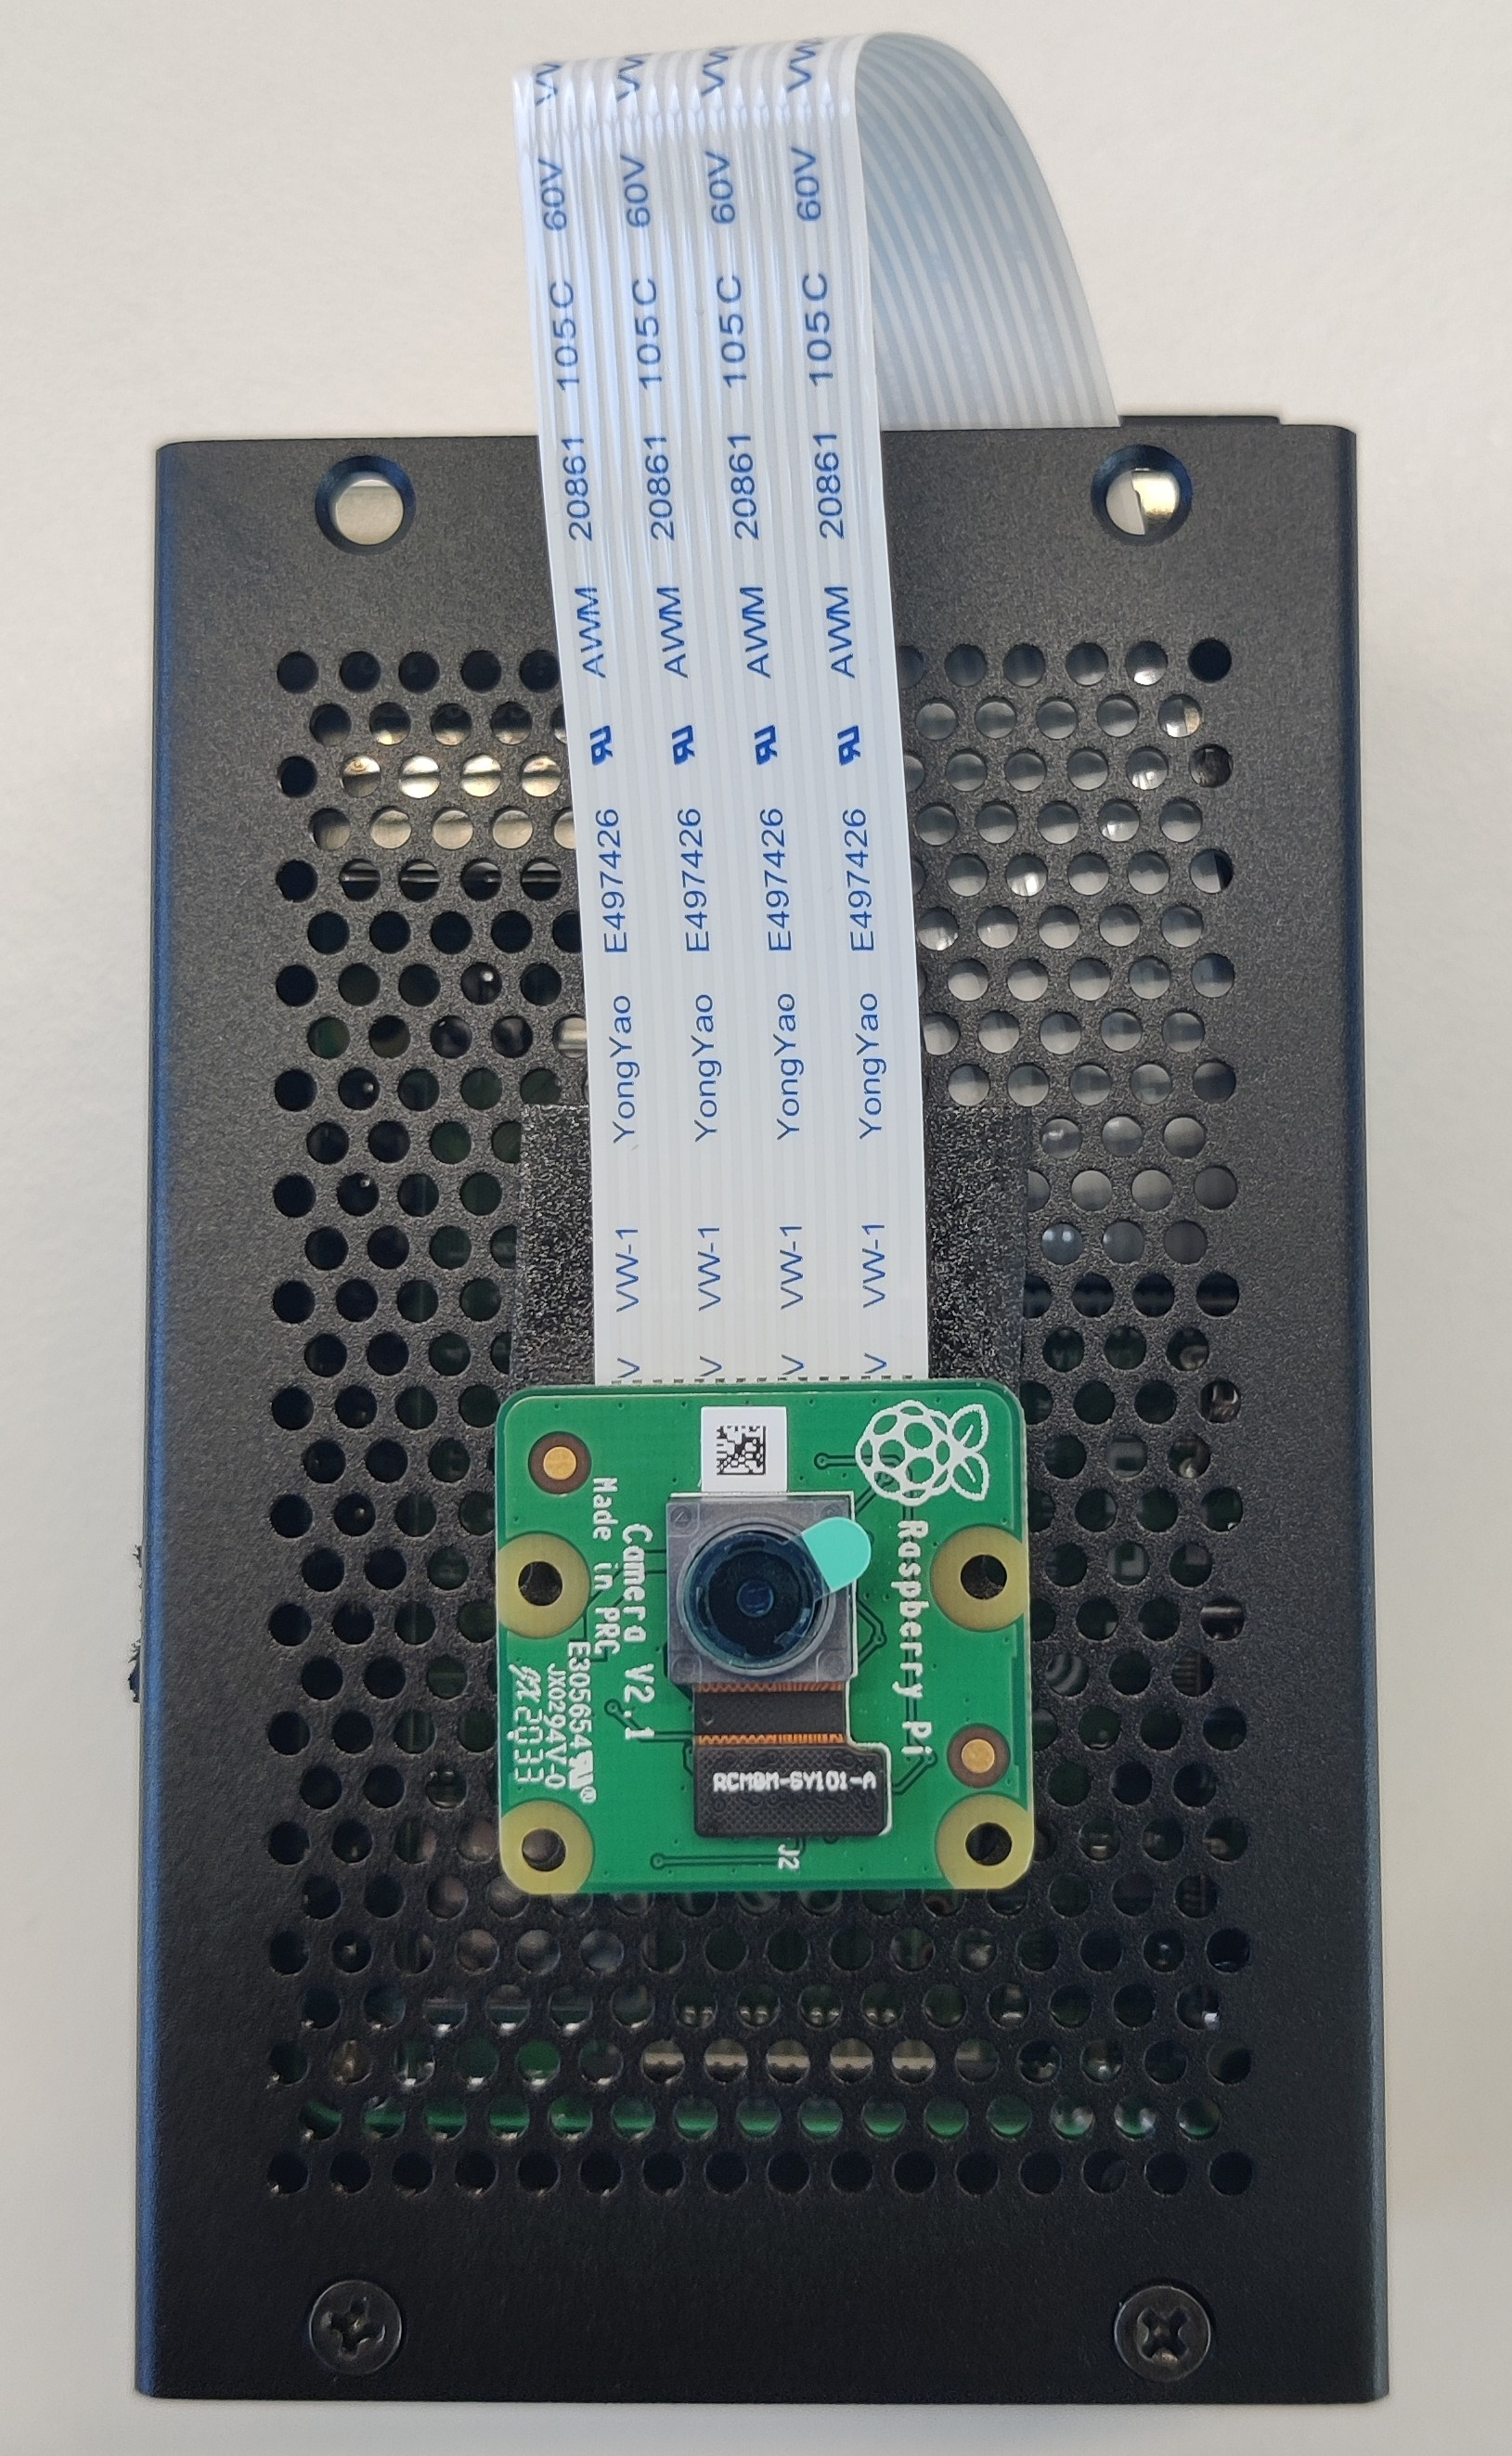
\includegraphics[scale = 0.07]{Master's thesis/images/RGB_camera.jpg} 
    \caption{The RGB Camera}
    \label{fig:AoA}
  \end{center}
\end{figure}  
However, instead of manually annotating these videos, the use cases of Machine Learning and Deep Learning are leveraged. With the advancement of Machine Learning and Deep Learning libraries, object detection and object recognition can be done with accuracy as high as 99\%. This field of Artificial Intelligence that trains computers to interpret and understand the visual world is called Computer Vision. With the advancement of AI and innovations in Deep Learning and Neural Networks, Computer Vision been able to take great leaps currently and has been able to surpass humans intelligence in some tasks related to detecting and labeling objects for optical sensors.


The RGB camera in the experiment and RADAR are mounted next to each other, so that the field of view of RADAR and camera overlaps. The camera used in this thesis captures 60 frames per second (fps). For the purpose of labelling the RADAR data, the scene is captured with an RGB camera alongside RADAR. The camera is connected to a 32-bit Raspberry pi 4. This Rpi leverages the camera to record videos. Each video file spans 1 second. The name of the file is the timestamp at which the file was created. As soon as the file is created, a parallel process dumps the data periodically to the AWS bucket. In order to prevent Rpi from memory overload, the files from the Rpi are removed as soon as they are dumped to AWS successfully. The important thing to notice here is the duration of the video. 1 sec is chosen so that it is easy later on to combine RADAR data as well RGB data. Once the data is dumped, the data is cleaned. For an instance, the videos of size 0 Kb are removed. These are the lost packets or the unsuccessful video captures.

\subsection{Platform for Collecting Data}
For this thesis, Data collected is huge. It is almost impossible for a local machine to run heavy computations on such a high volume of data. Therefore in order to run heavy computations without any memory leaks, the best possible technology available is the use of Cloud Resources. For the purpose of this thesis, we are using AWS EC2 instances. AWS EC2 instances are fast reliable and will be able to access the S3 buckets directly. 

There are different parameters to be taken into account while deciding to use CPU's or GPU's to train the deep learning models. Those parameters include the memory bandwidth, cost effectiveness and parallelism. GPU has on average better memory bandwidth in comparison to CPU's. Considering the data-set size, the larger the data-set the more advantage the GPU will have over CPU. As for the Parallelism of the model, some models have more parallelism than others. For example, Fast Forward Neural Networks (FNNs) and Convolutional Neural Networks (CNNs) can support high parallelism, therefore, it can be applied better on a Single Instruction Multiple Data (SIMD) processor such as the GPUs. Finally, coming to Cost-effectiveness, the power cost of GPU is higher than the CPU. For non parallel processes or less parallel processes like Recurrent Neural Networks, it is better to use a CPU. In this work, the cloud instances based on CPU or GPU is used to train the models according to the needs as mentioned above.

For this thesis, Deep Learning Base AMI Ubuntu instance of type p2.xlarge is used. Deep learning instance is launched in order to use the GPU instances for running the Deep Learning models. P2 instances provide up to 16 NVIDIA K80 GPUs, 64 vCPUs and 732 GiB of host memory, with a combined 192 GB of GPU memory, 40 thousand parallel processing cores, 70 teraflops of single precision floating point performance, and over 23 teraflops of double precision floating point performance ~\ref{amazonec2}. 


\subsection{Computing on Cloud for RGB Data}
\label{Computing on Cloud for RGB Data}

The data collected from RGB data which is stored in S3 buckets can be directly accessed from EC2 instance as both the instance and the bucket are present in the same AWS region.  For this project a hybrid of  two techniques are used for object detection on the RGB data collected. 
\begin{enumerate}
    \item \textbf{YOLOv3} - YOLOv3 is chosen because it is extremely fast and accurate. The mAP of YOLOv3 is measured at .5 IOU  which is on par with Focal Loss but about 4x faster. YOLOv3 uses a few tricks to improve training and increase performance, including multi-scale predictions, a better backbone classifier, and more ~\cite{yolo_time}. YOLOv3 returns output in the form of pre defined 80 classes on which the model is trained. Here in this thesis, only person class is a matter of interest. In order to detect only human, the detection class of the YOLOv3 model has been manipulated.
    \item \textbf{Motion Detection} - This technique is used to detect motion in a scene. It is used because sometimes it is possible for a person to be occluded in the video. For an instance, consider a person half occluded behind the desktop monitor, or a scenario where there is only hand moving in front of camera, or where someone is half visible behind the door, for such scenarios YOLOv3 will fail because there are a lot of occlusions present in the same. Therefore for such cases, motion detection algorithm is used on the RGB camera data. When the movement is beyond a fix threshold, only then the algorithm returns presence, otherwise it ignores small movements, for e.g.., movement due to curtains or leaves of the plants are ignored. The approach is very simple and self intuitive. When the program starts, it will capture a called baseline image. The program will keep comparing the new frame with this baseline image. If there is a movement in the new frame, the contents of the image will be different and if this difference is beyond a certain threshold,  the program will return Presence.
\end{enumerate}

Once the data is cleaned into AWS, YOLOv3 and  Motion Detector are run on the RGB data collected. Every second of collected data contains 60 frames, so for every second YOLOv3 and Motion Detector generates 60 labels. In the Lighting industry, the requirement for getting the true labels is within few seconds. The accuracy of milliseconds is not required in lighting industry. Therefore, for the sake of simplicity and better results, the mode value of the 60 labels was taken for every second. 

After using this pipeline, the labels corresponding to every second of RADAR data is ready. Its worth noticing that there might be some inaccuracies in the labelling because of the difference in the angle of view. 

\subsection{Transformations on RADAR Data}
\begin{figure}[ht]
  \begin{center}
    % below the size of the figure has been reduced for example
    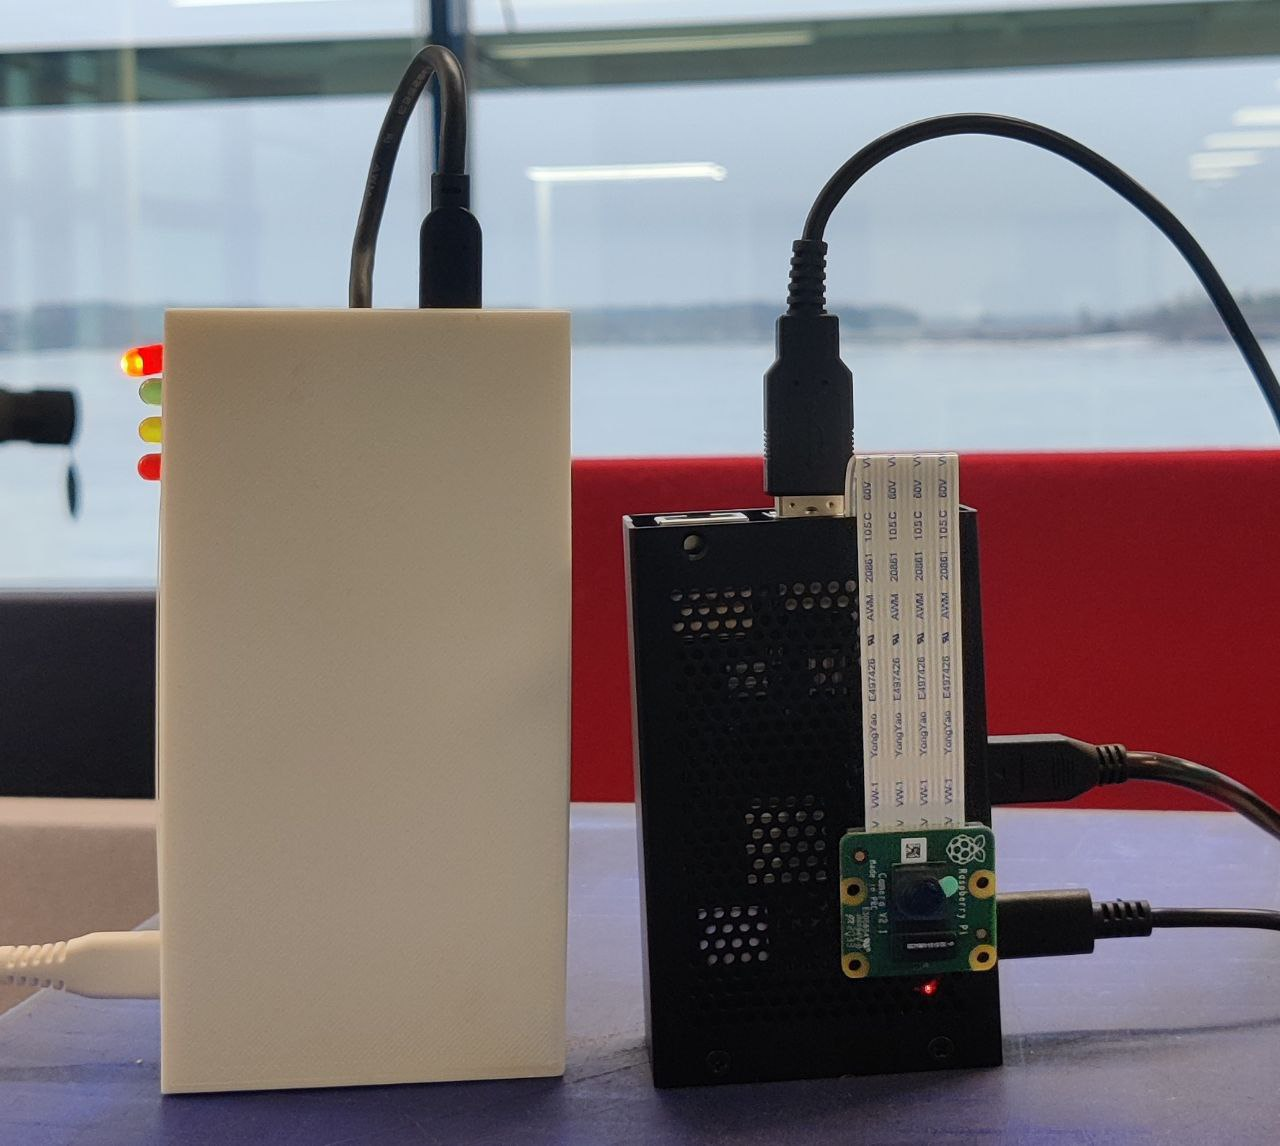
\includegraphics[width=0.5\textwidth]{Master's thesis/images/equipment.jpg} 
    \caption{RADAR and Camera}
    \label{fig:AoA}
  \end{center}
\end{figure}  
In the previous section, we talked about how the pipelines are arranged for the proper flow of data. In this section, we will talk about how the data is arranged for the machine learning model to work efficiently. This section will also explain the operations and transformations done on the data. In addition to that, we will see exploratory data analysis done on the radar data.

The data from FMCW RADAR is generated in the form of chirps/sweeps. According to the hardware configuration of the RADAR used in this thesis, it generated 497 samples in one chirp. Since the RADAR have two receiver antennas, it generates 497 per antenna in 1 chirp. RADAR generates 1 chirp is approximately 31.25 ms, although the time may vary in fractions of milliseconds. This means the RADAR generates approximately 32 samples in 1 second. On the other hand, the RGB camera operates at 60 fps. In order to overlap the data and make an effective labelling, the data from 32 chirps of RADAR is combined together to make a combined signal of 1 second. Alternately, it can be imagined that one instance of data for our Machine Learning/Deep Learning model corresponds to 1 sec of data, i.e. 32 sweeps from the RADAR and 60 frames of camera are mapped together. Therefore the data signature of the RADAR of 1 second can be imagined as a 3D matrix where first dimension corresponds to antenna number, second dimension corresponds to chirp number and the third dimension corresponds to Time. The value of cell is the actual amplitude of the signal. Timestamping is used for mapping of RADAR and RGB camera data. These 1 second videos of RGB camera when fed to YOLOv3 and Motion detector model, as explained in the previous subsection \ref{Computing on Cloud for RGB Data}, generates output in the form of True/False. 
\begin{figure}[ht]
  \begin{center}
    % below the size of the figure has been reduced for example
    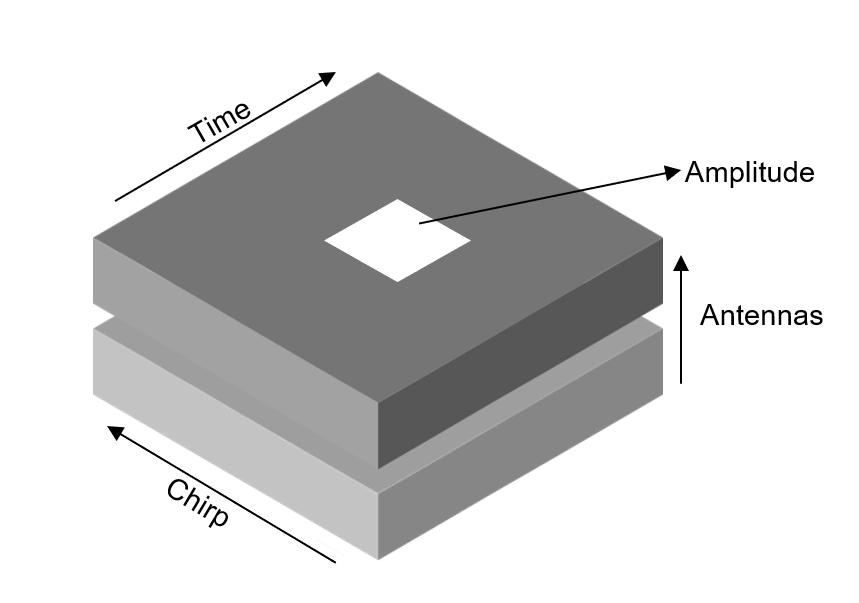
\includegraphics[width=0.5\textwidth]{Master's thesis/images/signature.PNG} 
    \caption{The data signature for RADAR}
    \label{fig:signature}
  \end{center}
\end{figure}  



In the Fig. \ref{fig:raw_signal}, random instances of RADAR data are sampled. Every plot corresponds to 1 second of data. The data from 32 chirps is flattened to make it a Time vs Amplitude plot. Since each chirp has 497 samples, therefore the Time axis has $32\times497$ samples on the x axis. The y axis corresponds to Amplitude of the received signal. The title of the subplots presents if there was presence or absence in the RADAR view. False corresponds to absence while Presence corresponds to Presence. Clearly there is significant difference between presence and absence. The signals from absence scenario is similar across time, or we can say that time does not change the signal. However it is completely different in presence scenario, the signal tend to change a lot over time.

\begin{figure}[ht]
  \begin{center}
    % below the size of the figure has been reduced for example
    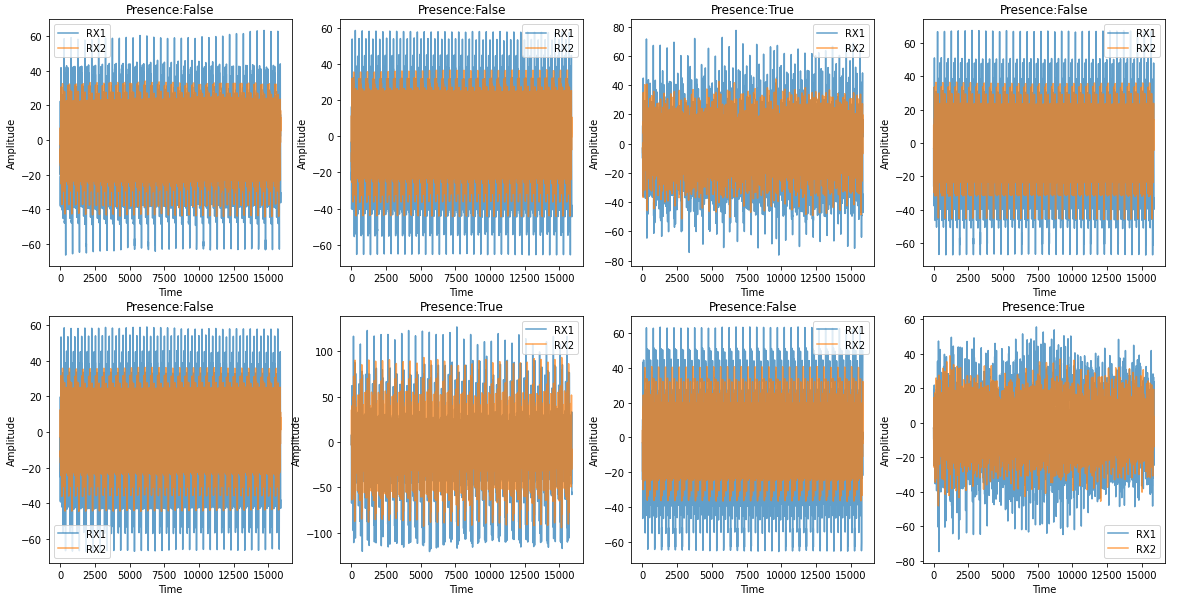
\includegraphics[width=01\textwidth]{Master's thesis/images/raw_signal.PNG} 
    \caption{Random sampling of 1 second of RADAR data}
    \label{fig:raw_signal}
  \end{center}
\end{figure}  

Deep learning models were tried directly using this raw data. However the model prediction was not highly accurate. One reason could be significant difference in amplitude in different scenarios. The amplitude differs a lot based on the range, and range of objects varies from scenario to scenario. Therefore the raw data can not be used directly for ML models. The second reason for not using this raw data directly for ML model is the maximum range capacity. The RADAR data in its raw form can detect objects up to 250 metres. But in an office environment, we really do not need data beyond some threshold. The data beyond this threshold will be just noise. The third reason is, the data in raw form has a lot of noise due to cluttering. The SNR for raw data is heavily compromised in raw form. Therefore, some transformations were required on this data for the ML model to work properly.

As explained in subsection \ref{Signal Processing for FMCW}, the data was converted from $Time\times Amplitude$ to $Range\times Amplitude$ using Fourier Transformation. As explained earlier, Fourier Transformation converts the Time into Frequency. Since in FMCW RADAR frequency directly estimates the Range, that is why Time gets converted to Range. This transformation is called \textbf{Range FFT}. Here FFT means Fast Fourier Transformation, which is a faster method of computing Fourier Transformations of discrete signal.

A very common problem associated with FFT is \textbf{Spectral Leakage}. An estimation of a signal computed using FFT or DFT does not contain spikes and zeros like shown in Fig. \ref{fig:comp_fft}, instead it will have a dominant peak which is then smudged over several consecutive bins. It happens because of finite window of data as the data is never infinitely large. In order to cater to this problem, windowing functions are used to reduce the spectral leakage. In this thesis \textbf{Blackman Window} is used. It is designed to have close to the minimum leakage possible. The Blackman window is defined as,
\begin{equation*}
    w(n) = 0.42 - 0.5\cos(2\pi n/M) + 0.08\cos(4\pi n/M)
\end{equation*}
where \(M\) is the number of samples and \(n\) is the $n^{th}$ sample. It is also known as an apodization which means ``removing the foot", i.e. smoothing discontinuities at the beginning and end of the sampled signal or tapering function \cite{blackman1958measurement}\cite{oppenheim2010discrete}.

Once the Blackman windowing is applied to raw data, FFT of the data is computed. The result of the FFT is then normalized to make the Euclidean norm of the signal equal to 1. Range FFT returns 512 samples( closest to 497), out of which half the samples are mirror images. But for the sake of putting an upper limit on the range i.e. to what range we want to detect objects, we have put an upper limit of 32 samples. This number 32 has been chosen after considerable number of experiments. These 32 samples corresponds roughly to 18.7 metres. 
\begin{figure}[ht]
  \begin{center}
    % below the size of the figure has been reduced for example
    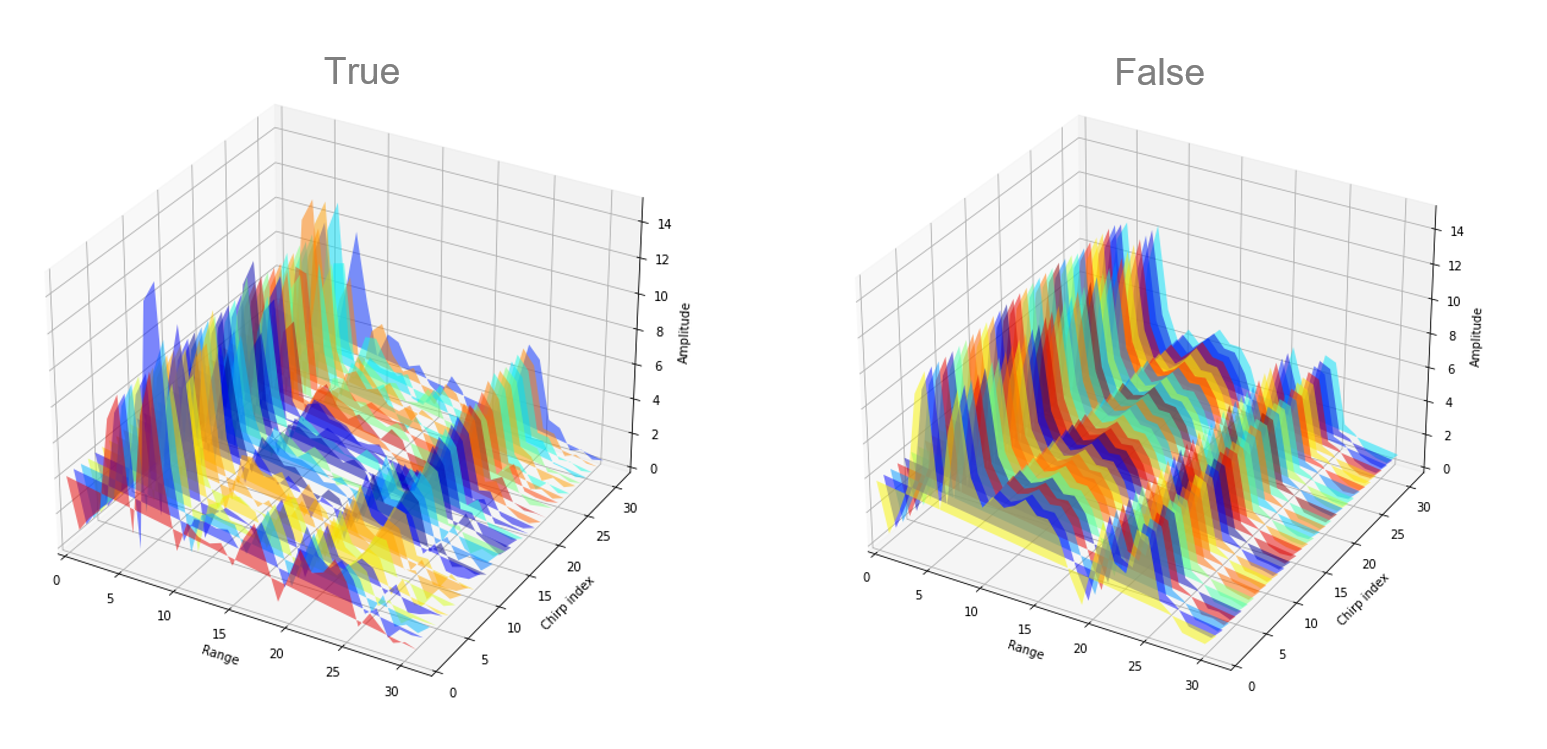
\includegraphics[width=1\textwidth]{Master's thesis/images/fft_p_a.PNG} 
    \caption{Range FFT comparison for human presence and absence with one receiver antenna}
    \label{fig:FFT_3d1a}
  \end{center}
\end{figure} 
Fig. \ref{fig:FFT_3d1a} represents a 3 dimensional view of Range FFT data. A comparison of the Range FFT signal for human presence and absence is done in the figure. It is worth mentioning that the plot indicates the Range FFT output of only one antenna. Similar signal is obtained from the another antenna as well. 
It is very evident from the plots that in the scenario when there was no human, the signal remain constant over chirps. However when there was human movement involved, the signal varies over chips.

\begin{figure}[ht]
  \begin{center}
    % below the size of the figure has been reduced for example
    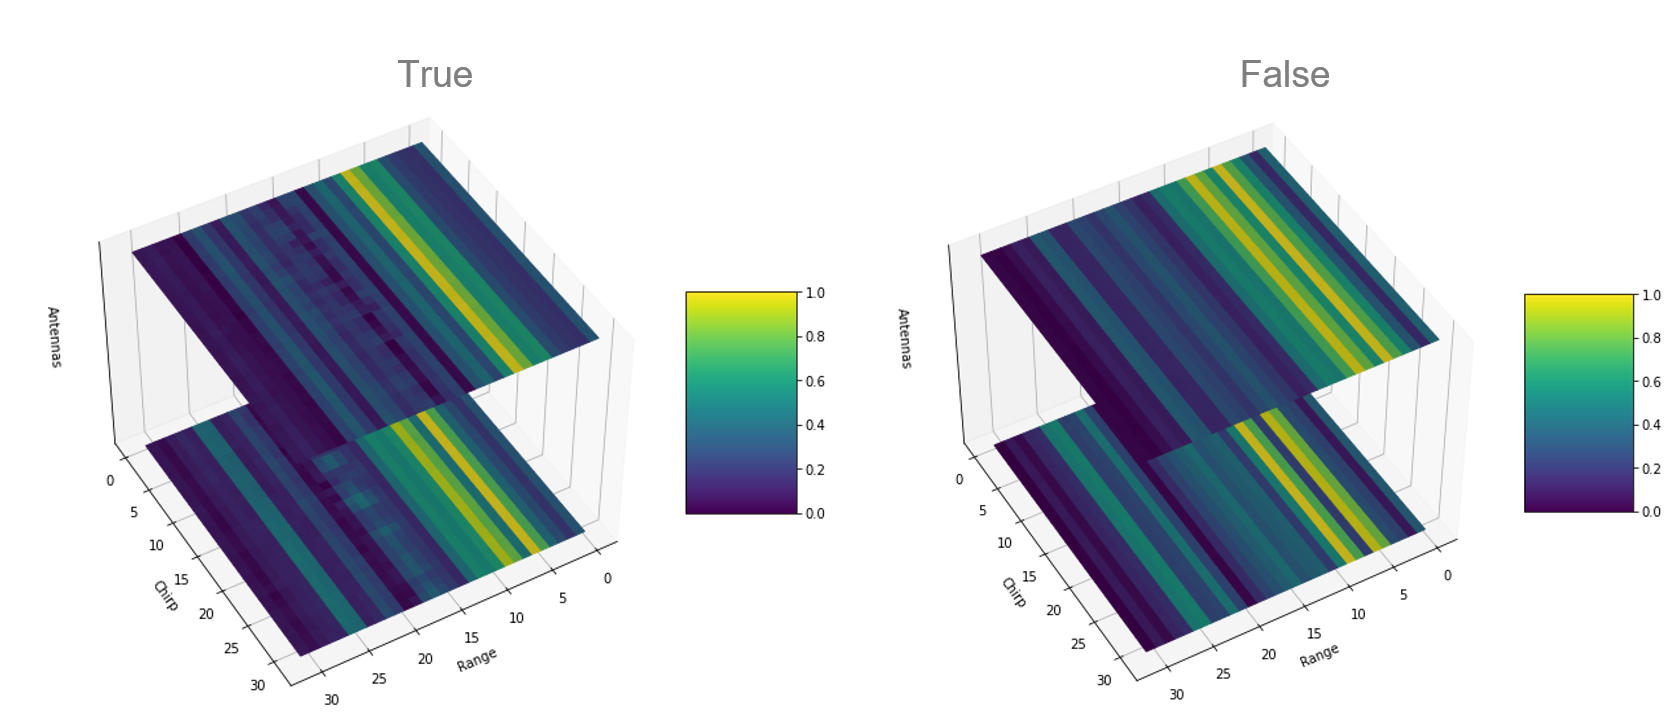
\includegraphics[width=1\textwidth]{Master's thesis/images/4d_fft.PNG} 
    \caption{Range FFT on random randomly sampled RADAR data}
    \label{fig:FFT_4d2a}
  \end{center}
\end{figure}   

To visualize this scenario even better, a 4 dimensional plot is drawn involving 2 antennas in Fig. \ref{fig:FFT_4d2a}. The color in the plots indicates the amplitude intensity. Yellow color corresponds to higher amplitude values and blue corresponds to lower amplitude values. It is evident in the plots that the amplitude values of the two antennas are always comparable in quantification. It can be seen in this plot as well that in the scenario of human absence, the amplitude of the signal remains constant across chirps. Comparatively in the human presence scenario, a distinctive smudge can be observed across chirps. This also comes by intuition that when the human movement in involved, a human body, which is a collection of points, is at different distance from the RADAR. It is important to note that the distance from one antenna is of course different than the distance from another antenna, but the difference is diminutive. 




\begin{figure}[ht]
  \begin{center}
    % below the size of the figure has been reduced for example
    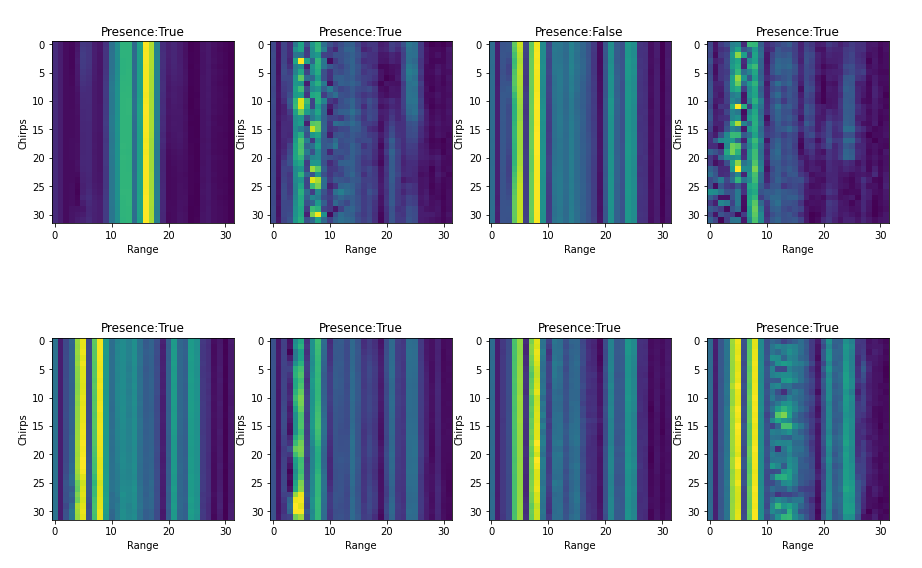
\includegraphics[width=01\textwidth]{Master's thesis/images/fft_1_antenna.PNG} 
    \caption{Range FFT on random randomly sampled RADAR data}
    \label{fig:FFT_plot}
  \end{center}
\end{figure}  

Random instances of the Range FFT are sampled. Fig. \ref{fig:FFT_plot} shows how data from Range FFT looks like. Every plot corresponds to 1 second of data. It i worth noticing that the y axis which corresponds to chirp index ranges from 0 to 32, and the Range axis also ranges from 0 to 32 on the x axis. 

\chapter{Experiments}
\label{chapter:methods}
\section{Test Rooms in Office Buildings}
\begin{figure}[ht]
  \begin{center}
    % below the size of the figure has been reduced for example
    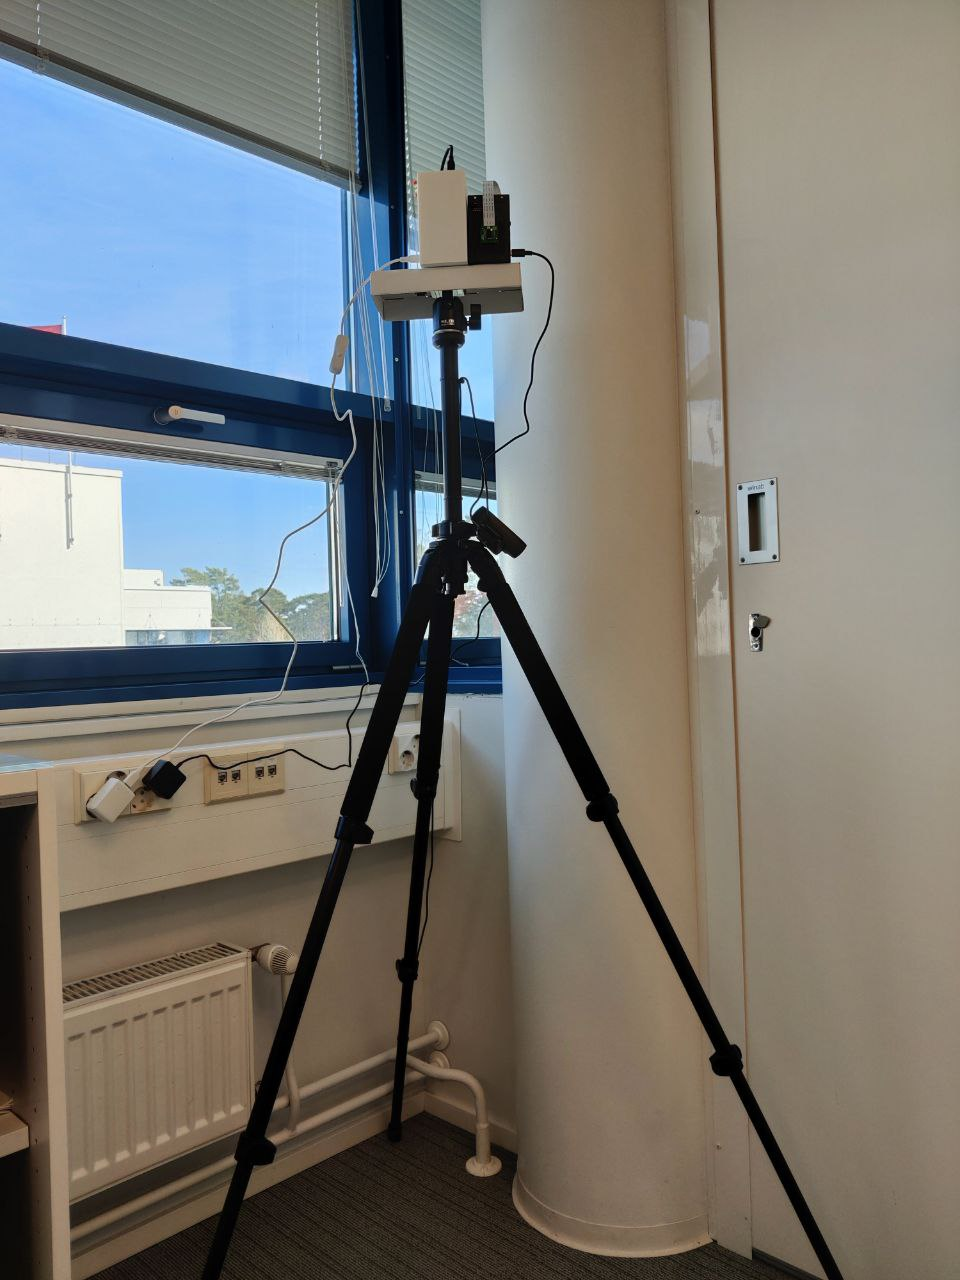
\includegraphics[width=0.6\textwidth]{Master's thesis/images/setup.jpg} 
    \caption{Setup}
    \label{fig:AoA}
  \end{center}
\end{figure}  
\section{Baseline Algorithm}
\label{section:environments}

\section{Advance Deep Learning Algorithms}
\label{section:environments}

\section{Results}
\chapter{Results}
\label{chapter:implementation}

You have now explained how you are going to tackle your problem. 
Go do that now! Come back when the problem is solved!

Now, how did you solve the problem? 
Explain how you implemented your solution, be it a software component, a
custom-made FPGA, a fried jelly bean, or whatever.
Describe the problems you encountered with your implementation
work. Sometimes the content of the environment chapter is combined
together with the implementation chapter.

 
\chapter{Conclusion and Future Work}
\label{chapter:discussion}

At this point, you will have some insightful thoughts on your
implementation and you may have ideas on what could be done in the
future. This chapter may be combined together with the evaluation
chapter. All the new insights and findings are given here!  This
chapter is a good place to discuss your thesis as a whole and to show
your professor that you have really understood some non-trivial
aspects of the methods you used\ldots




% Load the bibliographic references
% ------------------------------------------------------------------
% You can use several .bib files:
% \bibliography{thesis_sources,ietf_sources}
\bibliography{sources}


% Appendices go here
% ------------------------------------------------------------------
% If you do not have appendices, comment out the following lines
\appendix
\chapter{First appendix}
\label{chapter:first-appendix}

This is the first appendix. You could put some test images or verbose data in an
appendix, if there is too much data to fit in the actual text nicely.

For now, the Aalto logo variants are shown in Figure~\ref{fig:aaltologo}.

\begin{figure}
\begin{center}
\subfigure[In English]{
\includegraphics[width=.8\textwidth]{images/aalto-logo-en}}
\subfigure[Suomeksi]{
\includegraphics[width=.8\textwidth]{images/aalto-logo-fi}}
\subfigure[På svenska]{
\includegraphics[width=.8\textwidth]{images/aalto-logo-se}}
\caption{Aalto logo variants}
\label{fig:aaltologo}
\end{center}
\end{figure}


% End of document!
% ------------------------------------------------------------------
% The LastPage package automatically places a label on the last page.
% That works better than placing a label here manually, because the
% label might not go to the actual last page, if LaTeX needs to place
% floats (that is, figures, tables, and such) to the end of the 
% document.
\end{document}
